\documentclass[bwprint]{gmcmthesis}
\usepackage{amsmath}
\usepackage{url}
\numberwithin{figure}{section}
\renewcommand{\thefigure}{\arabic{section}-\arabic{figure}} 
% \documentclass[withoutpreface,bwprint]{cumcmthesis}
% 去掉封面与编号页

\title{中国研究生数学建模竞赛论文标题}
\baominghao{B104} %参赛队号
\schoolname{南京理工大学/自动化学院}%学校名称
\membera{白宇铖} %队员A
\memberb{李文睿} %队员B
\memberc{马寅锐} %队员C
\begin{document}
 \maketitle
 \begin{abstract}
概述
在SIR模型的基础上,本文建立了SLIRS模型。建立的SLIRS(Susceptible-Latent-Infectous-Removed-Susceptible)模型是一个随机隔间模型,每一个隔间中的个体都会以一定的概率转换到另一个隔间。
模型尽可能多地考虑了真实情况下的因素:
首先,加入了密切接触者(病毒携带者)、因病去世者、住院患者;
将感染者分成有症状感染者和无症状感染者,无症状患者可以自愈而有症状患者需要占用床位或使用药物;
引入人口结构考虑不同人群对病毒的抵抗力;引入接触矩阵,可以模拟政府的防控措施;
模型还考虑到了疫苗提供的免疫力,并且根据疫苗接种情况和疫苗现有效力将人群划分成了12类。
\par 针对问题一,本文采用改进的SIRDT模型对美国2022年1月1日至2022年4月10的奥密克戎数据进行拟合,并将由BFGS求得的参数带入到上海市疫情的SIR模型中,
对上海自2022年3月1日起的疫情数据进行了预测。
\par 针对问题二,首先用贝叶斯方法估计出有效再生数为。。。,然后调整接触矩阵用SLIRS模型模拟出疫情曲线,累计病例数为。。。
\par 针对问题三,首先依据现有政策,修改模型参数和接触矩阵,使用SLIRS模型进行模拟,得到疫情感染峰值为。。。清零时间为。。。
\par 最后,基于模型预测出的结果,我们总结出了一些有利于控制病毒传播的策略,并写成给上海政府的建议书。



\keywords {疫情预测\quad  隔间模型\quad SIR\quad SLIRS\quad 接触矩阵}
\end{abstract}

%\pagestyle{plain}

%目录
\tableofcontents

\section{问题背景与问题重述}
\subsection{问题背景}
2019年底爆发的新冠肺炎疫情给全人类带来深重苦难,至今已有4亿多人感染,6000多万人死亡。面对突如其来的疫情,中国政府始终将人民生命财产安全放在第一位,果断采取科学防控措施,有效遏制了疫情大面积蔓延,有力改变了病毒传播的危险进程,最大限度保护了人民生命安全和身体健康。直至2022年初,我国的新冠肺炎疫情已得到基本控制。
\par 然而,在2022年3月上海突然爆发了奥密克戎疫情,直到现在疫情仍未得到根本控制,使得疫情防控态势又紧张了起来。面对疫情,需要我们采取科学防控措施,利用已经公布的相关数据和数学模型,对本轮上海新冠肺炎疫情进行预测,使人们更好的认识新冠肺炎传播规律,也能为相关部门采取防控措施提供参考,对疫情防控具有积极作用。

\subsection{问题重述}
题目提示需要在分析上海市卫生健康委员会和国家卫生健康委员会通报的实时疫情数据的基础上(主要包括累计报告病例、累计治愈病例、累计死亡病例、跟踪隔离人数、单日新增确诊病例等),建立新冠肺炎传播模型以预测未来疫情发展趋势并评估防疫策略。
\begin{enumerate}
\item
问题1:搜集有关美国国内疫情应对措施,分析在此防控措施下造成的美国疫情蔓延态势。若上海采取相同防控措施,通过建立模型分析疫情蔓延情况及可能带来的严重后果。
\item 问题2:疫情爆发初期,上海市政府采取精准防控策略并公布了相关数据,需要分析上述数据以建立数学模型预测在该措施下的再生数。通过前面建立的模型预测两个月内疫情发展趋势和累计病例数。
\item 问题3:随着疫情发展趋势,上海市政府加强了管控措施,积极推行如:全员核算、启用方舱医院接收轻型患者和无症状感染者等措施。需要根据对应的公布数据,建立恰当的数学模型预测包括:流行时间、流行规模等指标在内的本次疫情发展趋势。预测完成后还需要根据五月份的数据来验证模型的有效性。若上海疫情在五月中旬之后仍未结束,需要根据模型预测一周内疫情发展趋势。
\item 问题4:根据建模结果,总结出一些对抗击疫情有积极作用的针对性建议,给有关部门进行参考。
\end{enumerate}



\section{模型假设}
\par 以下对本文中的模型进行一些基本的假设
\begin{enumerate}
\item 假设气候因素(温度、湿度)对病毒传播无影响
\item 假设人口总数在预测区间内恒定
\item 假设个体对病毒的易感性相同
\item 假设病毒传染性不变
\item 以一天作为模型的最小时间单元
\end{enumerate}

\par 其中针对经典的SIR模型及其变种,还有以下额外的假设:
\begin{enumerate}
    \item 易感者与患病者有效接触即被感染,变为患病者,可被治愈变为康复者,无潜伏期,有终身免疫力。
\end{enumerate}
    

\section{符号说明}

\begin{tabular}{cc}
    \hline
    \makebox[0.2\textwidth][c]{符号}	&  \makebox[0.5\textwidth][c]{意义} \\ \hline
        $N_a$	    & 人口数 \\ \hline
       $S_a$	    & 易受新冠感染的未接种疫苗的人群 \\ \hline
       $E_a$	    & 携带病毒的人群 \\ \hline
       $I_{S,a}$	    & 有症状感染者,包括$I_{S,a}^{drug}$和$I_{S,a}^{naive}$\\ \hline
       $I_{S,a}^{drug}$	    & 服用药物的有症状感染者 \\ \hline
       $I_{S,a}^{naive}$	    & 未服用药物的有症状感染者 \\ \hline
       $I_{A,a}$	    & 无症状感染者 \\ \hline
       $H_a$	    & 住院患者,包括$H_{N,a}$和$ICU_a$ \\ \hline
       $H_{N,a}$	    & 住院(非ICU)患者 \\ \hline
       $ICU_a$	    & ICU患者 \\ \hline
       $D_a$	    & 去世人员 \\ \hline
       $R_a$	    & 康复者\\ \hline
       $V_{1,a}$	    & 接种了第一剂疫苗,且第一剂疫苗尚未生效的人群 \\ \hline
       $V_{1,a}^{e}$	    & 接种第一剂疫苗且第一剂有效的人群 \\ \hline
       $V_{2,a}$	    & 接种了第二剂疫苗,且第二剂尚未生效的人群 \\ \hline
       $V_{2W,a}^{e}$	    & 接种第二剂疫苗且第二剂有效的人群 \\ \hline
       $V_{2W,a}$	    & 接种第二剂疫苗,且主要疫苗接种保护已经减弱了六个月的人群 \\ \hline
       $V_{B,a}$	    & 接种加强剂且加强剂尚未生效的人群 \\ \hline
       $V_{B,a}^{e}$	    & 接种加强剂且加强剂已生效的人群 \\ \hline
       $V_{BW,a}$	    & 接种加强剂疫苗,且加强剂疫苗的保护已经减弱的人群 \\ \hline
       $R_{a}^{V}$	    & 已接种疫苗且从感染中恢复的的人群 \\ \hline
       $\lambda_{a}(t)$	    & t时刻感染率 \\ \hline
       $\beta$	    &传播率\\ \hline
       $\varphi$	    &由NPI导致的传输率降低值\\ \hline
       $r_a$	    &对SARS-CoV-2的易感性\\ \hline
       $M_{a,\tilde{a}}$	    &个人与个人的平均每日接触次数\\ \hline
       $\frac{1}{\gamma_E}$	    &潜伏期的平均持续时间(天)\\ \hline
       $\frac{1}{\gamma_I}$	    &平均感染期(天)\\ \hline
       $k$	    &无症状个体相对于有症状个体的传染性\\ \hline

      
   \end{tabular}

   \begin{tabular}{cc}
       \hline
       \makebox[0.2\textwidth][c]{符号}	&  \makebox[0.5\textwidth][c]{意义} \\ \hline
          
   
          $\frac{1}{\gamma_{SH}}$	    &从症状出现到住院的平均时间(天)\\ \hline
          $\frac{1}{\gamma_{HD}}$	    &从住院(非ICU)到死亡的平均时间(天)\\ \hline
          $\frac{1}{\gamma_{UD}}$	    &从ICU入院到死亡的平均时间(天)\\ \hline
          $\frac{1}{\gamma_{HR}}$	    &康复前住院时间(天)\\ \hline
          $\frac{1}{\gamma_{UR}}$	    &康复前的ICU住院时间(天)\\ \hline
          $p_a^s$	    &出现症状的未接种疫苗感染的年龄相关比例\\ \hline
          $p_a^h$	    &需要住院治疗的未接种症状性感染的年龄相关比例\\ \hline
          $p_a^{HD}$	    &未接种疫苗的住院(非ICU)患者的年龄相关死亡率\\ \hline
          $p_a^{UD}$	    &未接种ICU患者的年龄相关死亡率\\ \hline
          $p_a^{icu}$	    &需要ICU的未接种疫苗住院患者的年龄相关比例\\ \hline
   
   
          $\frac{1}{\omega_1}$	    &第一剂给药和第一剂完全保护之间的平均间隔(天)\\ \hline
          $\frac{1}{\omega_2}$	    &第一剂完全保护与第二剂给药之间的平均间隔时间(天)\\ \hline
          $\frac{1}{\omega_3}$	    &第二剂给药和第二剂完全保护之间的平均间隔(天)\\ \hline
          
          $\frac{1}{\omega_P}$	    &第二剂完全生效和给予增强剂之间的平均间隔(天)\\ \hline
          $\frac{1}{\omega_4}$	    &接种增强针和增强针完全生效之间的平均间隔(天)\\ \hline
          $\frac{1}{\omega_B}$	    &加强针完全有效和加强失效之间的平均间隔(天)\\ \hline
          $\frac{1}{\omega_R}$	    &从先前感染中获得的保护的平均持续时间(天)\\ \hline

          $S\left( t \right) $    & $t$时刻预测的易感人数(人)  \\ \hline
          $I\left( t \right) $ 	& $t$时刻预测的感染人数(人)  \\ \hline
          $R\left( t \right) $ 	& $t$时刻预测的治愈人数(人)  \\ \hline
      \end{tabular}


\section{问题分析}
\subsection{对上海疫情情况的调研}
为了给对模型的分析提供参考,需要首先对上海疫情近期的发展情况以及政策变动进行调研。经过对近期新闻的搜集和整理,绘制疫情曲线和政策变动图如图\ref{sh}所示
\begin{figure}[!h]
\centering
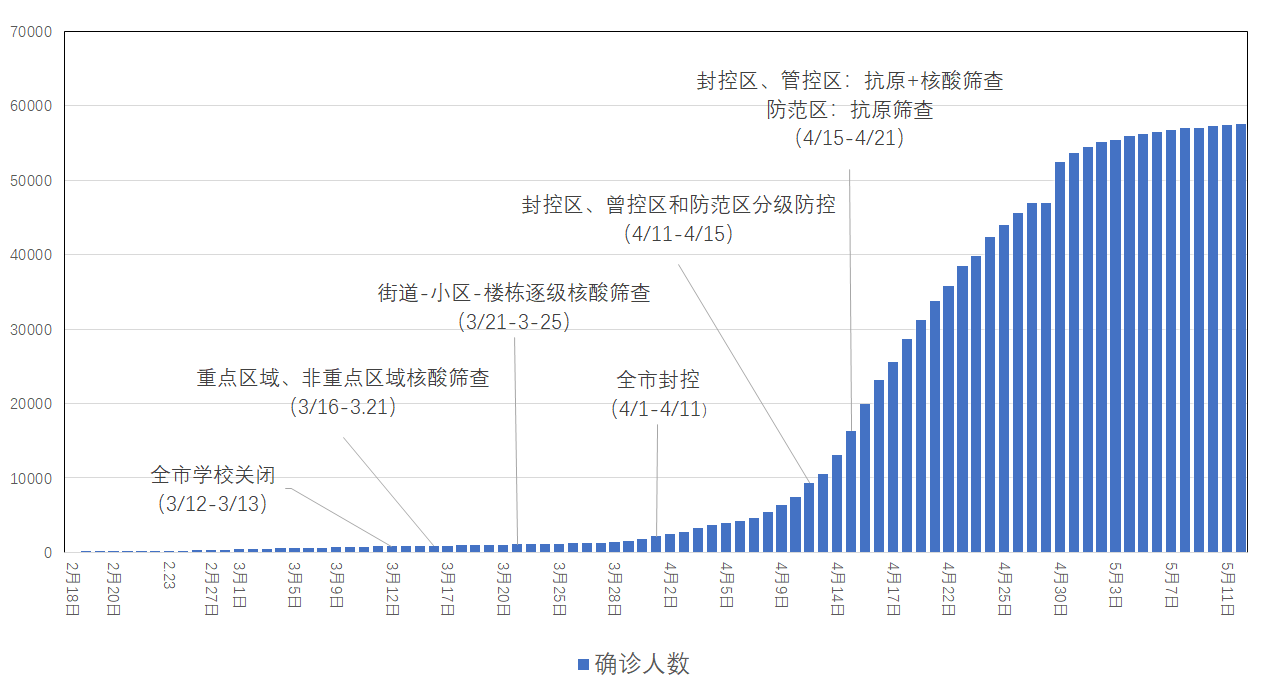
\includegraphics[width=.9\textwidth]{shanghai_bianhua.png}
\caption{上海防控政策的变化和疫情曲线}
\label{sh}
\end{figure}
\par 本轮奥密克戎疫情爆发以来,上海市陆续升级公共卫生干预措施对疫情进行管控。3 月12 日起,全市中小学调整为线上教学,幼儿园、托儿所停止入园,大学封闭。从3 月16 日起,对社区逐级开展“街镇-小区-楼栋”的区域化、网格化核酸筛查;3 月28 日5 时起浦东、浦南及毗邻区域实施封控,开展核酸筛查;4 月1 日开始全市封控;4 月10 日后划分封控区、管控区和防范区进行分级防控,因地制宜采取不同的防疫检测和防控措施。
\subsection{对问题一的分析}
问题一要求预测出上海在采取美国式“躺平”防疫政策的情况下会出现的疫情情况。首先我们需要对美国的防控策略进行调查,并利用现有的美国疫情数据推算出模型参数。最后将确定了参数的模型应用在上海的场景下,从而预测出可能的疫情规模。流程图如下所示
\subsection{对问题二的分析}
问题二要求根据上海市政府初期的精准防控策略,估计本次疫情的发展规模,并且估计在此策略下的再生数。首先根据上海的精准防控策略调整接触矩阵
\subsection{对问题三的分析}
问题三要求预测在上海实施了严格防疫管控措施的情况下的疫情趋势。

\section{数学模型}
\par 在传染病研究史中,多数研究都是依托疾病爆发早期数据,结合特定传染病传播规律,综合考虑国家预防
政策,拟合传染病传播模型,针对未来疾病可能爆发时间点,爆发峰值人数进行预测。通过此类预测结果帮助
国家政府提出进一步的防治政策。目前的主流研究方法通常分为传统方法、时间序列方法、机器学习方法等。
\par 传统方法通常包括SIR模型及其变种,通过建立了隔间模型来研究传染病传播规律;时间序列方法主要包括
ARIMA、EEMD等方法方法,可以很好地模拟传染病发病率在时间序列上的变动趋势,并对未来的发病率进行预测;
机器学习方法则通常是利用监督学习以寻找模拟参数,并根据干预措施评分对疾病的传播率做出预测。

\subsection{相关概念}
\subsubsection{再生数 Reproduction Number}
再生数通常指基本再生数与有效再生数

\par 基本再生数$R_0$:在流行病学中,基本再生数表示为$R_0$,代表的是在所有个体都为易感人群中一个感染病例所
直接产生的预期病例数,该定义假定没有其他人受到感染或免疫(自然或通过疫苗接种)。$R_0$并不是病原体的生物学常数,它还受到其他因素的影响,例如环境条件和受感染人群的行为。$R_0$值通常是从
数学模型估计的,估计值取决于所使用的模型和其他的参数值。
\par 有效再生数$R_t$:实际上,在任何特定时间,不同比例的人口对任何特定疾病都有免疫力。考虑到这一点,
提出了有效再生数$R_t$的概念。$R_t$是部分易感人群中单个感染个体在时间$t$引起的新感染的平均数。可以通过
将$R_0$乘以易感人群的比例$s\left( t \right)$来进行计算。
\par 基本再生数$R_0$不一定与有效再生数$R_t$相同。

\subsubsection{感染率 Force of Infection}
\par 感染率$lambda$:在流行病学中,感染率$lambda$是指易感个体感染传染病的比例,因为它考虑了易感性,
所以它可以用来比较统一传染病在不同人群之间,甚至不同传染病之间的传播率。也就是说,$lambda$与有效传播率
$beta$(Effective Transmission Rate)成正比。
\par 具体计算公式如下所示:
\begin{equation} \label{}
    \lambda =\frac{\text{新感染人数}}{\text{易感人群数量}\times \text{平均暴露时间}}
\end{equation}

\par 这样的计算存在一个显著的问题,那就是并非所有新感染都报告了,而且通常很难知道有多少易感者被暴露。
然而,如果假设人口的均匀混合和矩形人口分布(如发达国家普遍存在的人口分布),则可以计算当前情况下的
感染率,在这种情况下,$lambda$的计算公式如下所示:
\begin{equation} \label{}
    \lambda =\dfrac{1}{A}
\end{equation}
\par 其中$A$代表的是感染的平均年龄,换句话说,$A$也是是感染前在易感人群中花费的平均时间。


\subsubsection{隔间模型 Compartment model}
\par 隔间模型是一种非常通用的建模技术。它们经常被应用于传染病的数学建模。种群被分配到带有标签的隔间——例如$S$、$I$或$R$ ,
(易感人群、感染人群或恢复人群)。人群在隔间之间进行传播,其中标签的顺序通常显示隔间之间的流动模式,例如SEIS 表示易感、暴露、感染,然后再次易感。
\par 此类模型的起源是 20 世纪初,1916年的Ross、1917年的Ross和Hudson、1927年的Kermack和McKendrick和1956年的Kendall都为隔间模型作出了重要贡献。
\par 这些模型通常使用常微分方程运行,但也可以与随机框架一起使用,这更现实但分析起来更复杂。模型可以预测诸如疾病如何传播、感染总数或流行病持续时间等事物,并估计各种流行病学参数,例如繁殖数。这样的模型可以显示不同的公共卫生干预措施如
何影响流行病的结果,例如,在特定人群中 发布有限数量的疫苗最有效的技术是什么。


\subsection{SIR模型}
SIR模型是一种常见的描述传染病传播的数学模型,其基本假设是将人群分为以下三类:

\begin{itemize}
    \item 易感人群(Susceptible):指未得病者,但缺乏免疫能力,与感病者接触后容易受到感染。对与COVID-19而言,除去易感染者和康复者,几乎所有人都是易感者。
    \item 感染人群(Infective):指染上传染病的人,他可以传播给易感人群。
    \item 移除人群(Removed):被移出系统的人。因病愈(具有免疫力)或死亡的人。这部分人不再参与感染和被感染过程。
\end{itemize}

SIR模型的基本表达式:
\begin{equation} \label{}
\begin{aligned}
        &\frac{dS\left( t \right)}{dt}=-\frac{\lambda S\left( t \right) I_p\left( t \right)}{N}\\
        &\frac{dI\left( t \right)}{dt}=\frac{\lambda S\left( t \right) I_p\left( t \right)}{N}-\mu I\left( t \right)\\
        &\frac{dR\left( t \right)}{dt}=\mu I\left( t \right)\\
\end{aligned}
\end{equation}

\par 其中:
\begin{equation} \label{}
    N\,\,=\,\,S\left( t \right) +I\left( t \right) +R\left( t \right) 
\end{equation}

\par 其具体流程图如下图所示:
\begin{figure}[!h]
\centering
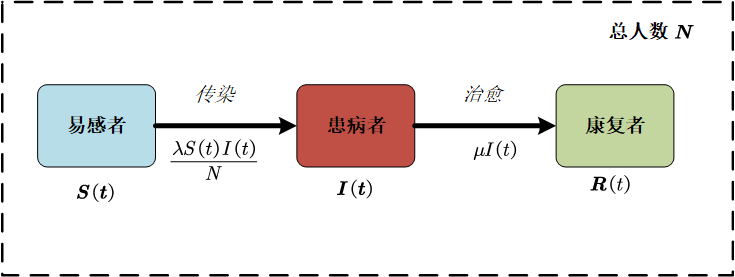
\includegraphics[width=.7\textwidth]{./SIRMODEL.png}
\caption{SIR传染病模型传播示意图}
\label{fig1}
\end{figure}

\subsection{SIRDT模型}
\par 此为本文提出的SIR模型的拓展模型,美国自2020年3月开始,已经累计死亡了102万人,占到了美国总人口数的0.3$\%$。为了保证拟合、预测效果的准确性,我们
将模型优化为了SIRDT模型,其相对于经典的SIR模型主要有以下两点改动:

\begin{enumerate}
    \item 总人数$N$不再是固定不变的,而是会根据累计的死亡数据动态调整。我们假定除COVID-19造成的死亡以外的所有出生、死亡数据能够保持均衡。
    \item 增加了因COVID-19死亡的人群$D$(Death)。
\end{enumerate}

\par 其中我们用于计算参数的SIRDT模型公式如下所示:

\begin{equation} \label{}
    \begin{cases}
        \dfrac{dS\left( t \right)}{dt}\,\,=\,\,-\dfrac{\lambda S\left( t \right) I\left( t \right)}{N\left( t \right)}\\
        \dfrac{dI\left( t \right)}{dt}\,\,=\,\,\dfrac{\lambda S\left( t \right) I\left( t \right)}{N\left( t \right)}-\mu I\left( t \right)\\
        \dfrac{dR\left( t \right)}{dt}\,\,=\,\,\mu I_p\left( t \right)\\
        N\left( t \right) \,\,=\,\,N-D_r\left( t \right)\\
    \end{cases}
\end{equation}

\par 其中累计死亡人数我们不再另设参数来计算,而是直接使用利用采集到的美国疫情的死亡数据,而在上海的感染人数的计算值中,由于累计死亡人数目前是578人
占到上海总人口数的0.0022$\%$,所以我们在上海市的感染人数预测中暂时忽略死亡人数对总人数的影响。

\par 综上所述,所以其实我们最后使用了两个模型,一个考虑死亡人数来计算更精确的模型参数,一个根据实际情况忽略死亡人数的影响。

\par 其中$N$为美国的总人口数,$D\left( t \right)$为当日累计的死亡数据。

\par 改进后的SIRDT模型的传播示意图如下图所示:

\begin{figure}[!h]
    \centering
    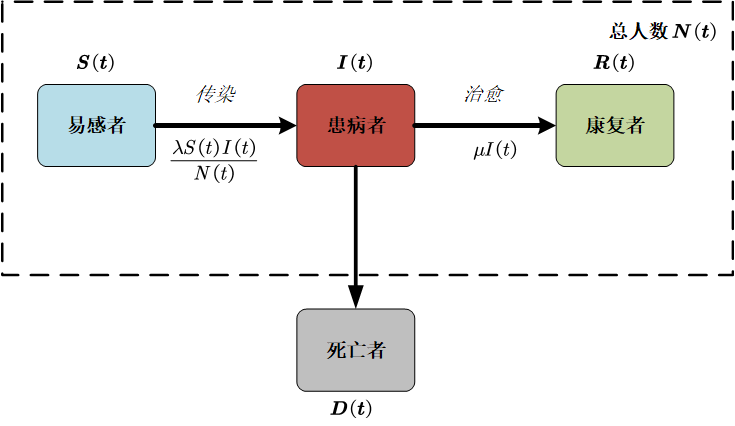
\includegraphics[width=.7\textwidth]{./SIRDTMODEL.png}
    \caption{SIRDT传染病模型传播示意图}
    \label{fig1}
\end{figure}


\subsection{SLIRS模型}
SLIRS(Susceptible-Lantent-Infectious-Removed-Susceptible)模型是对SIR模型的拓展。相比于基础的SIR模型,SLIRS主要考虑到病毒携带者、因病去世者的存在以及康复者可能会反复感染。将人群分成了以下几种:
\begin{enumerate}
\item 易感人群(Susceptible)$S$指会被感染的人群
\item 病毒携带人群(Lantent/Exposed)$E$指与感染者接触,但尚未感染的人群。这一类人群没有传染性,但会在一定时间内变为感染者。
\item 感染者(Infectious)$I$指被病毒感染的人群,这类人一定具有传染性。根据症状有无,可以进一步分成无症状感染者(asymptomatic infectious)$I_a$和有症状感染者(symptomatic infectious)$I_s$。无症状感染者一般情况下不需要住院就能自愈,变为康复者;而有症状感染者根据病情严重性,在医疗资源足够的情况下,会进入普通病房或ICU病房
\item 康复者(Recovered)$R$指刚从感染状态恢复健康的人群。这一类人因为曾被感染因而对病毒有较高的免疫力,但随着时间发展,其免疫力会逐步下降,最终转变为易感人群。
\item 因病去世者(Deceased)$D$
\item 住院病人(Hospitalized)$H$,可进一步划分为普通病房(包含方舱医院)病人和ICU病房病人。基于合理假设,这一类人通常不再有传染性,但可能会因病离世。


\end{enumerate}

\par 本文模型考虑到了病毒在不同年龄段中的传播特性、致病率、致死率等特性的差异,按14个年龄段划分人群。在人群中展开疫苗接种,能产生一定免疫效果,降低致病率和致死率;与此同时,采用疫苗种类、接种剂数、疫苗免疫效果的时变特性会带来抗病毒效果的差异。因此,本模型同时将。。。考虑抗病毒药物的效果,。。。
\par 采用随机模型,符合二项分布。对每一个个体,其
\subsubsection{年龄段的划分}
由于奥密克戎病毒在不同年龄段呈现不同的感染率、重症率、致死率,同时,各年龄的疫苗接种情况有差异,所以,本模型考虑到了人口结构。
\begin{figure}[!h]
\centering
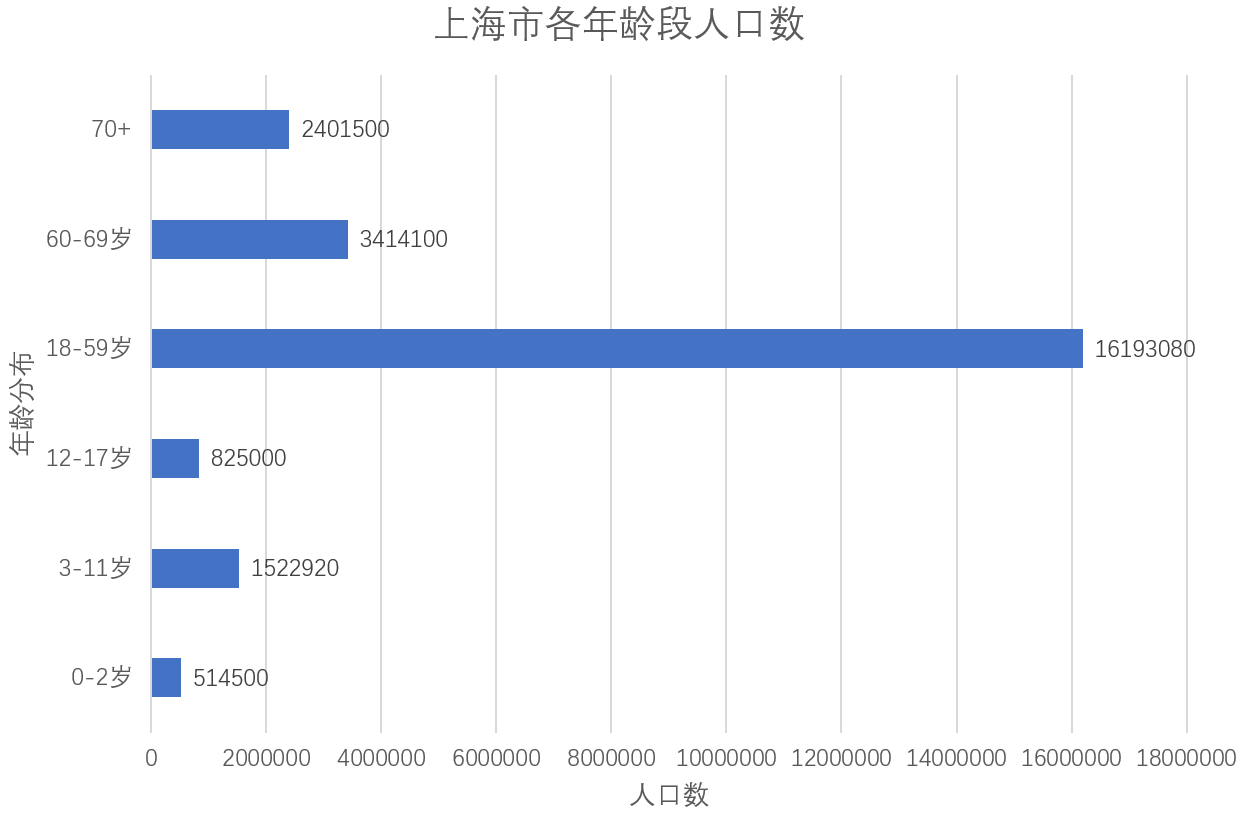
\includegraphics[width=.75\textwidth]{renkou.png}
\caption{上海人口结构}
\label{renkou}
\end{figure}

\subsubsection{接触矩阵}
接触矩阵表述了不同年龄人群之间的接触频次。接触矩阵每一点的值$CM_{ij}$表示年龄段$i$平均每天接触到年龄段$j$的人数。Dina等人的论文\cite{}给出了对中国人口接触矩阵的估计。

\par 因此,我们可以通过调整接触矩阵的值来模拟政府的管控措施,如图\ref{cm}分别绘制了无疫情期间、关闭学校、关闭学校和工作场所、全市封控情况下的接触矩阵。可见,一般情况下,同龄人之间的接触最为频繁,因而矩阵对角线上及其周围的值较大;在封闭学校的情况下,青少年年龄段的接触减少;全市封控的情况下,整个矩阵的元素值均大幅减小。

\begin{figure}[!h]
\centering
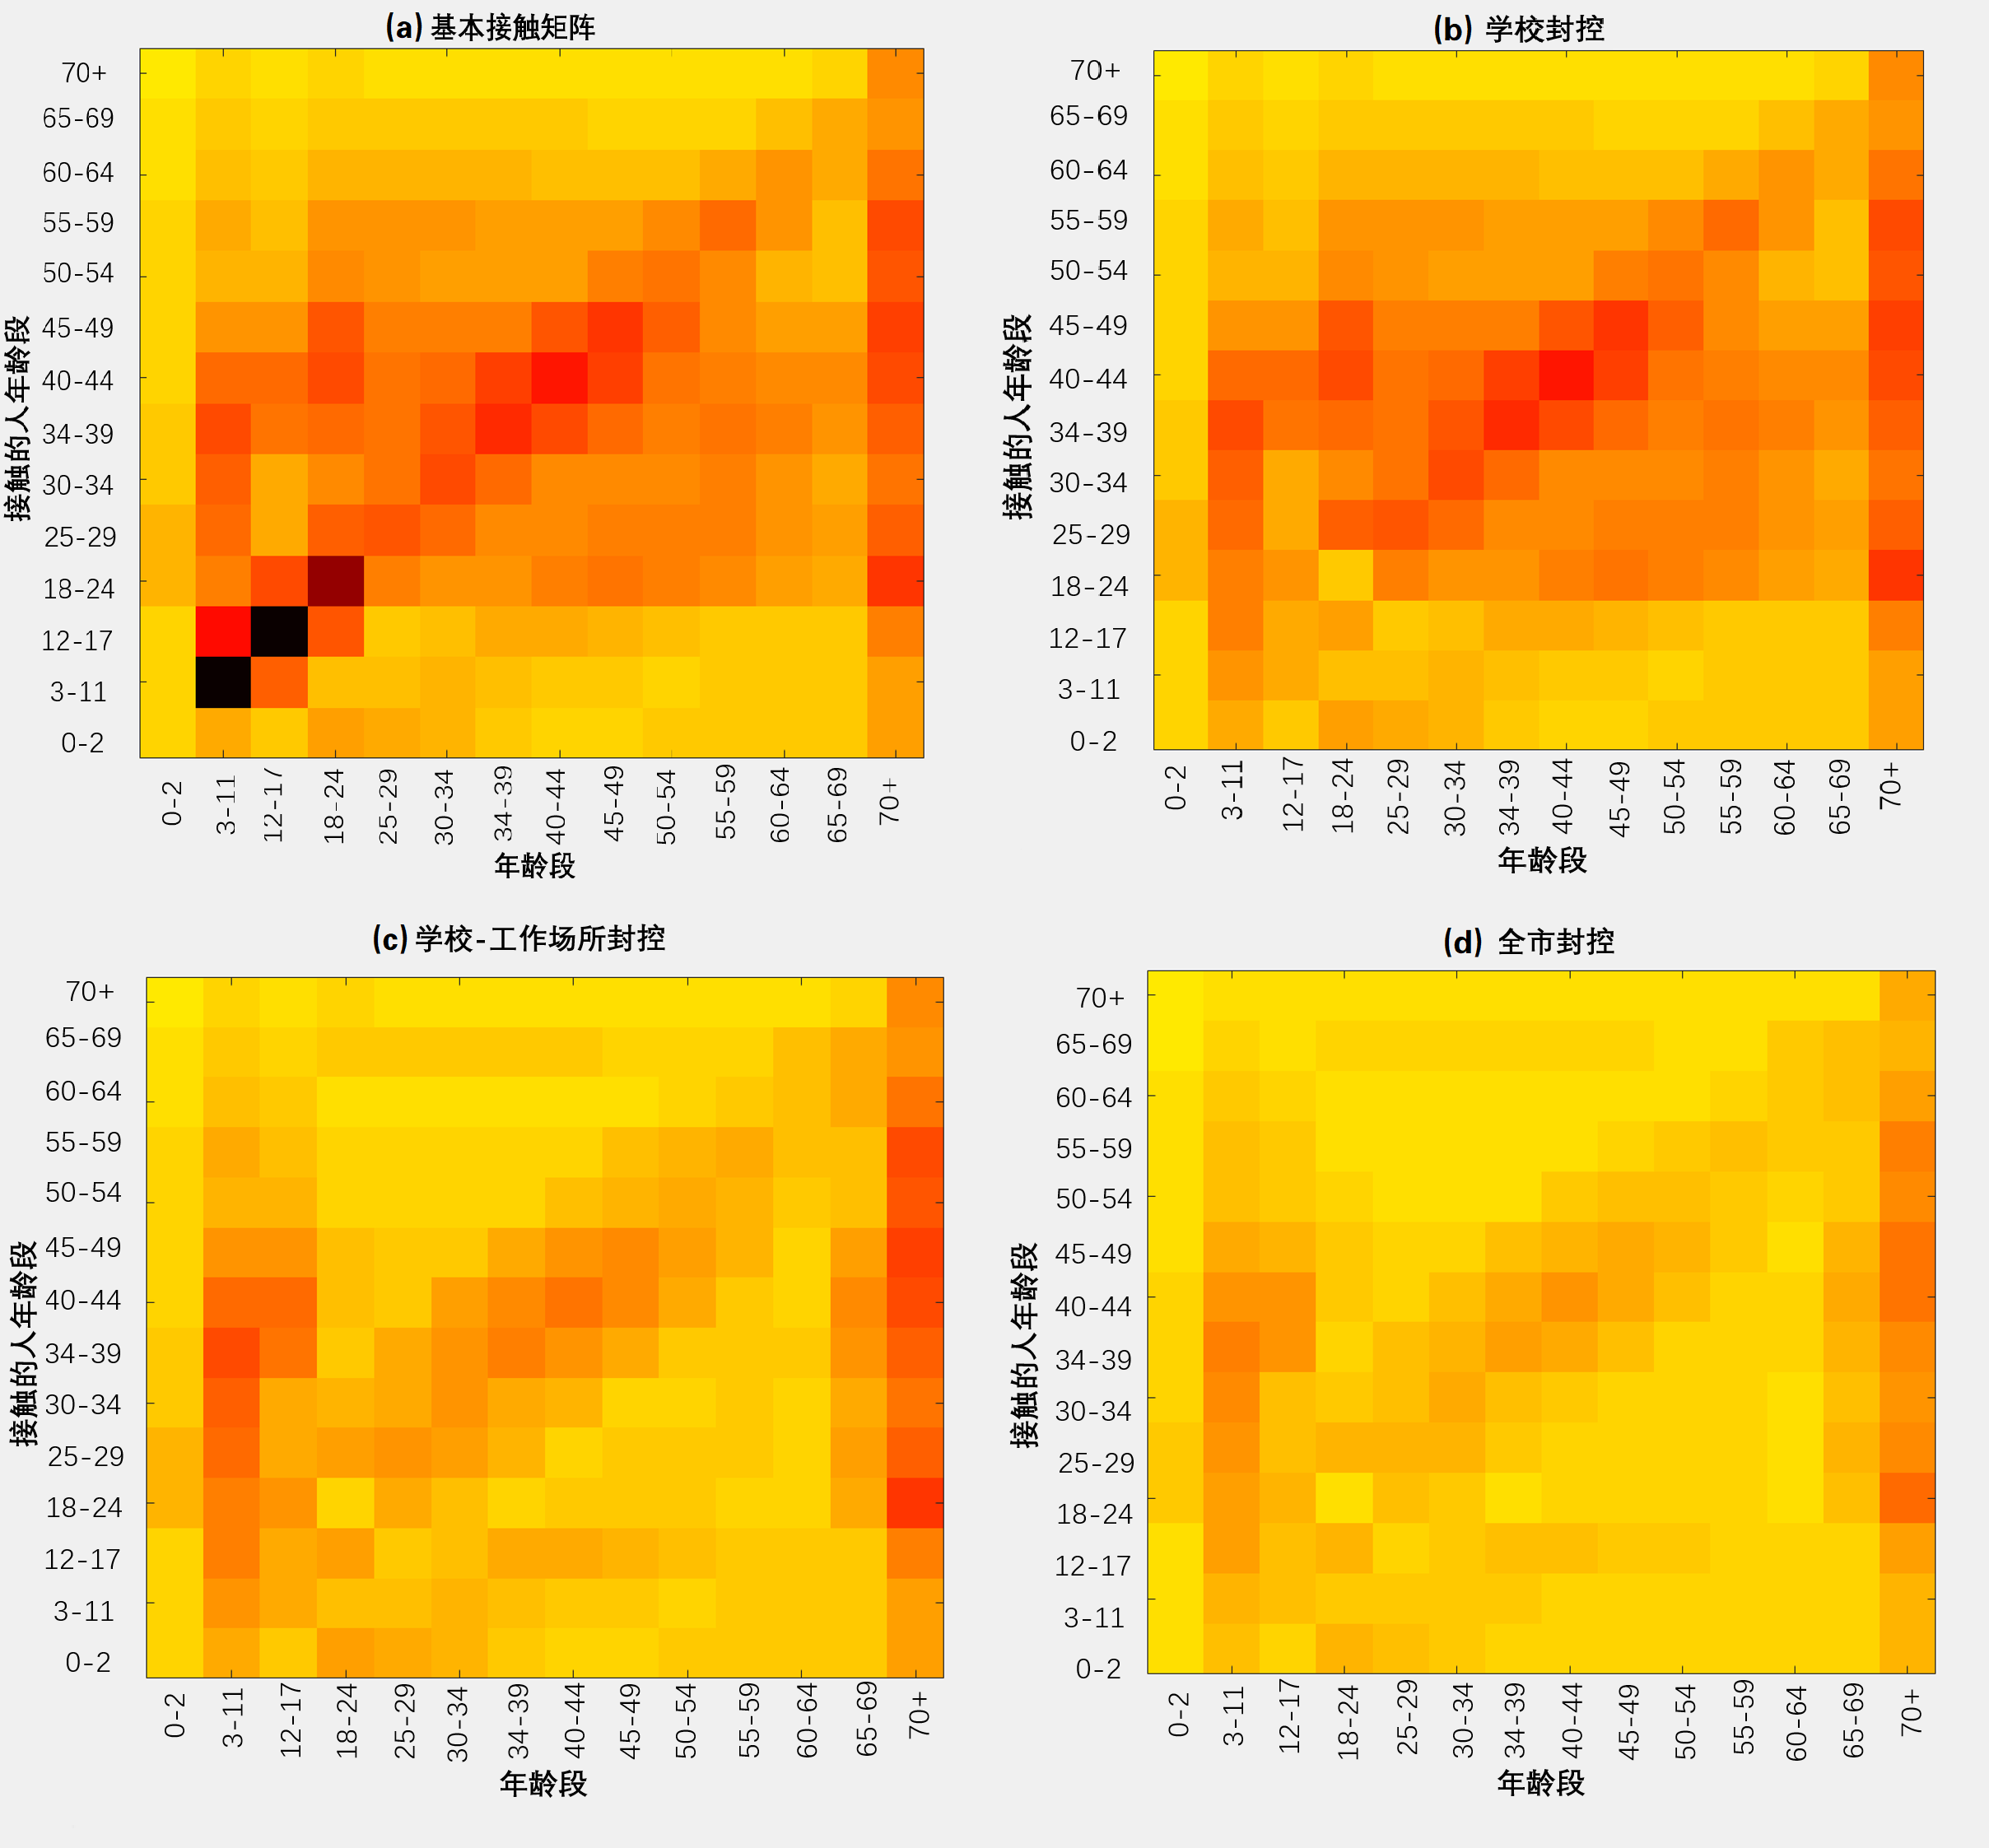
\includegraphics[width=1\textwidth]{4CM.png}
\caption{接触矩阵}
\label{cm}
\end{figure}
%\begin{figure}[!h]
%\centering
%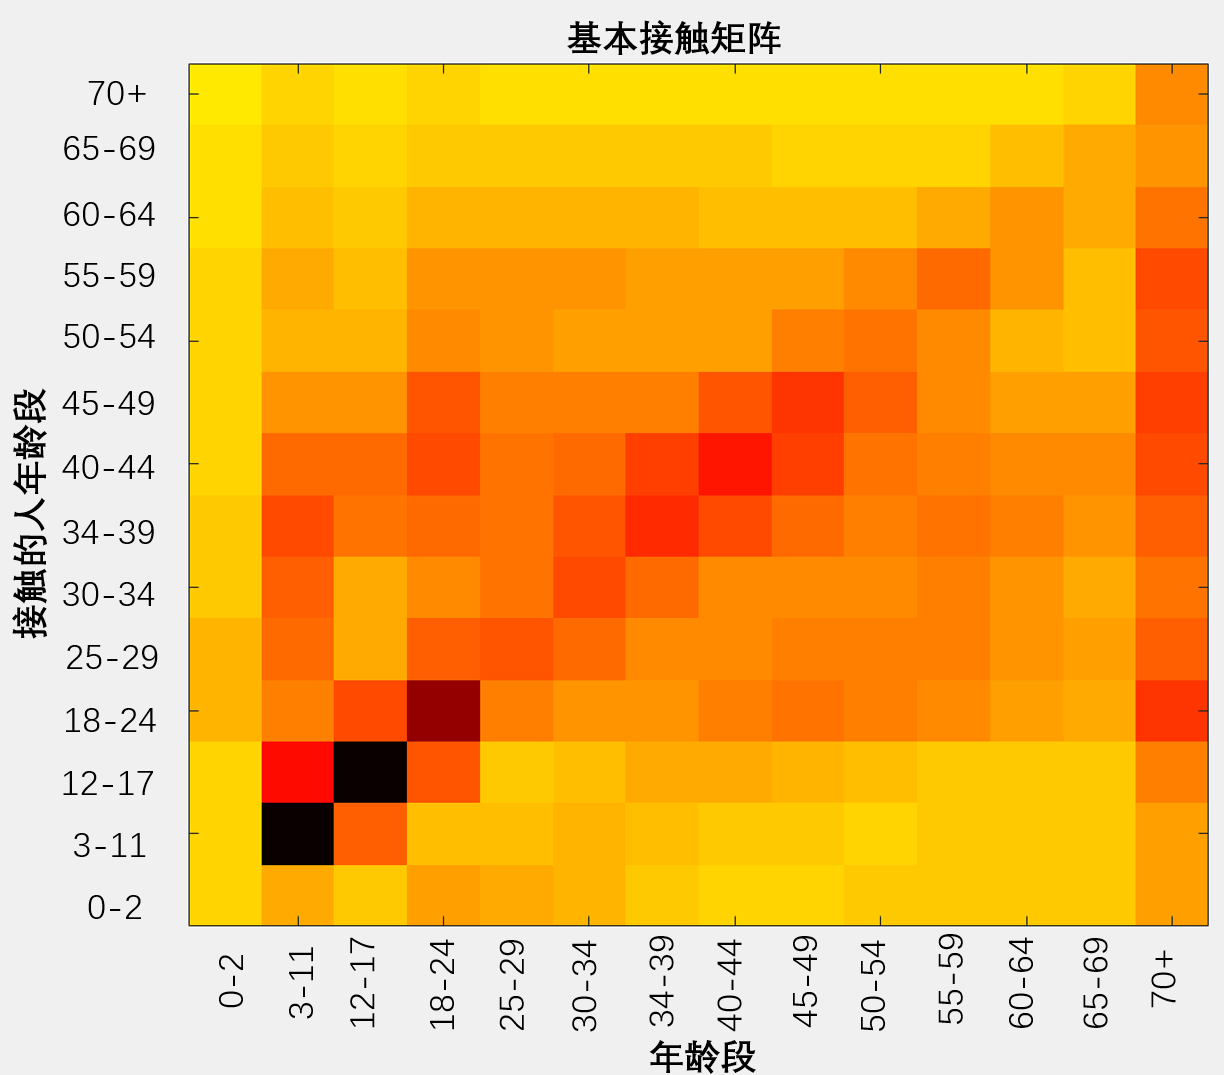
\includegraphics[width=.75\textwidth]{baseCM.png}
%\caption{上海防控政策的变化和疫情曲线}
%\label{hos}
%\end{figure}
%
%\begin{figure}[!h]
%\centering
%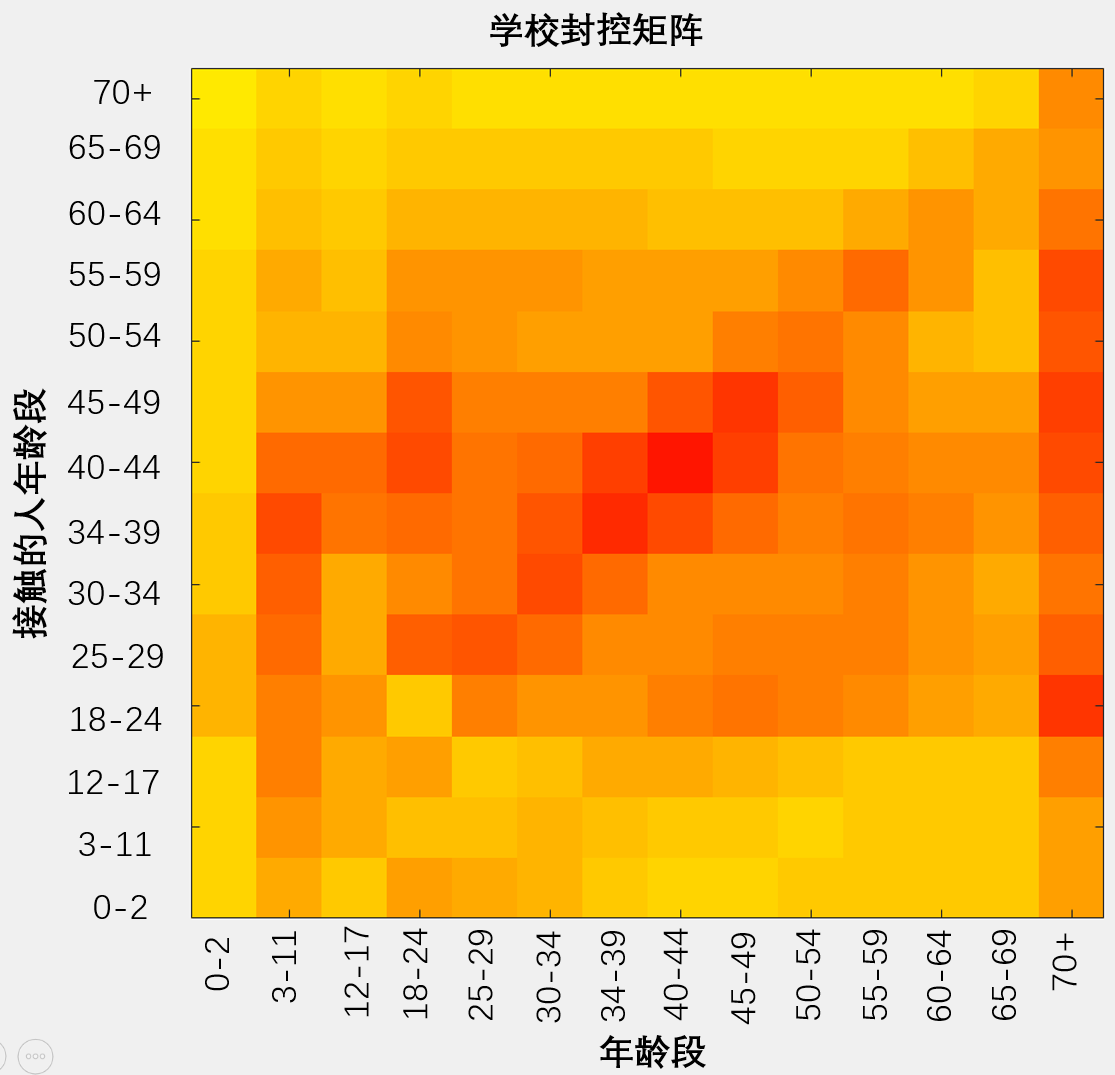
\includegraphics[width=.75\textwidth]{sCM.png}
%\caption{上海防控政策的变化和疫情曲线}
%\label{hos}
%\end{figure}
%
%\begin{figure}[!h]
%\centering
%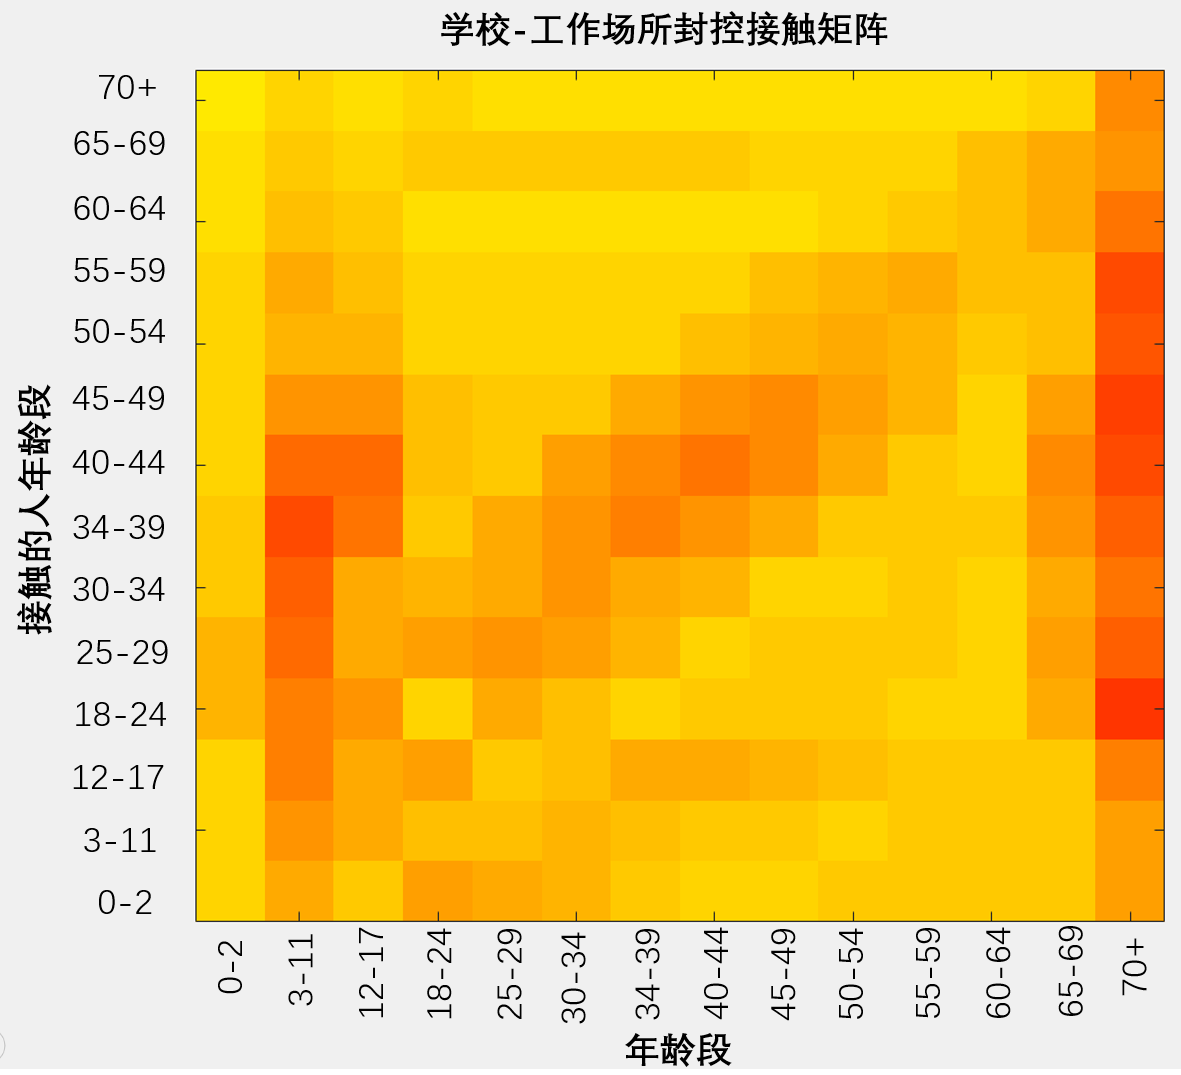
\includegraphics[width=.75\textwidth]{swCM.png}
%\caption{上海防控政策的变化和疫情曲线}
%\label{hos}
%\end{figure}
%
%\begin{figure}[!h]
%\centering
%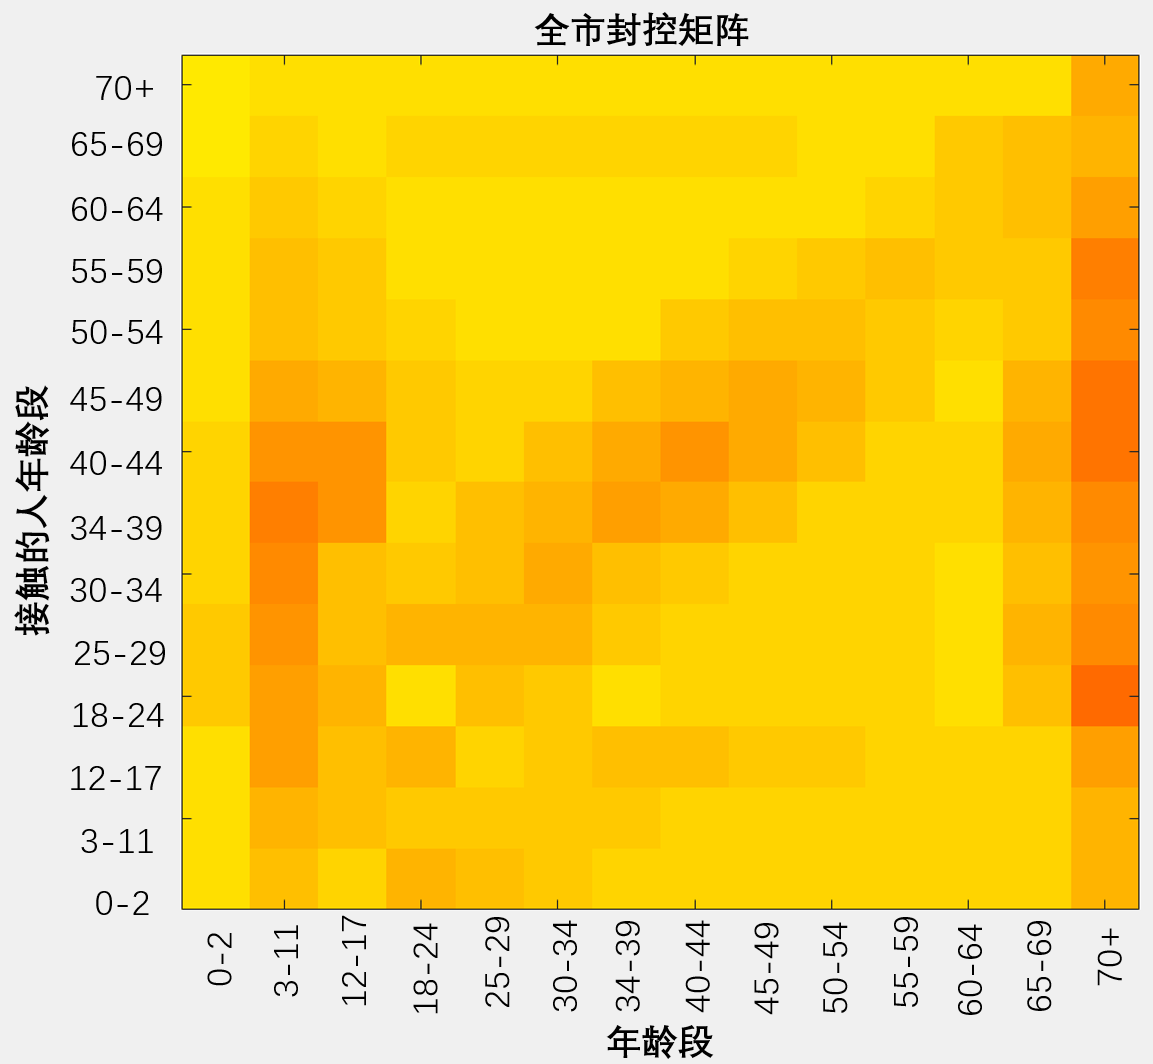
\includegraphics[width=.75\textwidth]{cityclose.png}
%\caption{上海防控政策的变化和疫情曲线}
%\label{hos}
%\end{figure}
\subsubsection{隔间模型状态转变的随机链式过程}
\begin{figure}[!h]
\centering
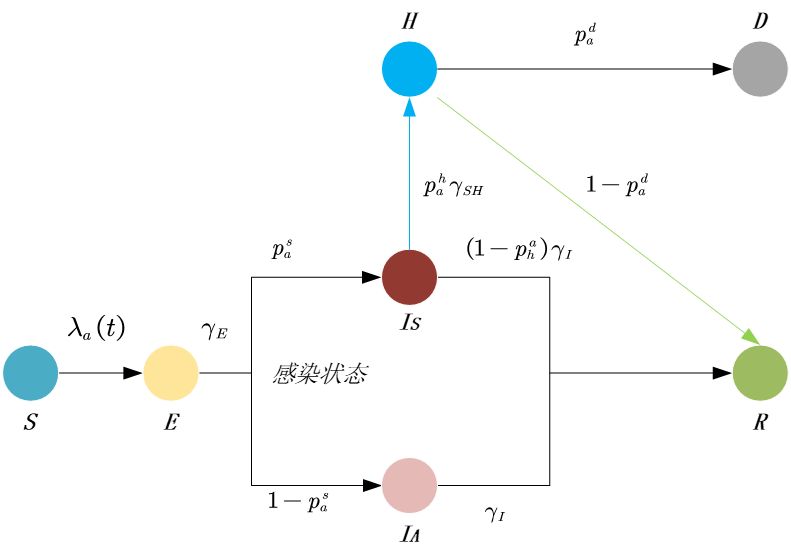
\includegraphics[width=.75\textwidth]{seirhd.png}
\caption{状态转移图}
\label{SLIRS}
\end{figure}

如图\ref{SLIRS}所示,易感人群$S$到暴露人群(病毒携带者、密切接触者)$E$的转移概率由FOI(感染率)$\lambda_a$决定,针对每一个易感者个体,其转移概率为
\begin{equation}
p(E_a\vert S_a)=\lambda_a=1-\exp(-\lambda_aV_e^{inf}) 
\end{equation}
$\lambda_a$与接触矩阵有关,其表达式为
\begin{equation}
  \lambda_a(t)=\frac{1}{T}\sum_jCM_{aj}\cdot\beta\frac{I}{N}
\end{equation}
\par 人群$E$平均经过$1/\gamma_E$时间会转变为病毒感染者$I$,每个个体的转移概率为
\begin{equation}
p(I_a\vert E_a)=\frac{1}{\gamma_E}
\end{equation}
\par 在病毒感染者中,占$p_a^s$比例的为有症状感染者$I_s$,其余为无症状感染者。结合考虑疫苗的有效性,$E$中个体转移到$I_S$的概率为
\begin{equation}
p(I_{S,a}\vert E_a)=\frac{1}{\gamma_E}p_a^s(1-\epsilon^{inf})
\end{equation}
转移到$I_A$的概率为
\begin{equation}
p(I_{A,a}\vert E_a)=\frac{1}{\gamma_E}(1-p_a^s)(1-\epsilon^{inf})
\end{equation}
其中,$\epsilon^{inf}$表示由于疫苗免疫力的存在,个体抗感染的能力。
\par 无症状感染者不需要就医,平均康复时间为$\gamma_I$,有症状感染者中有$p_a^h$比例的人会经平均$\gamma_{SH}$时间被转运至医院。因此可以推算出,感染者自然康复的概率为
\begin{equation}
\begin{aligned}
&p(R\vert I_{A,a})=\frac{1}{\gamma_I}\\
&p(R\vert I_{S,a})=\frac{1}{\gamma_I}(1-p_a^h)
\end{aligned}
\end{equation}
有症状感染者住院的概率为
\begin{equation}
p(H_{a}\vert I_{S,a})=\frac{1}{\gamma_{SH}}p_a^h
\end{equation}
\par 就医人群$H$不再具有传染性,因病死亡(转移到$D$)的概率为
\begin{equation}
p(D\vert H_a)=p_a^d
\end{equation}
康复(转移到$R$)的概率为
\begin{equation}
p(R\vert H_a)=1-p_a^d
\end{equation}
\par 根据每个个体状态转换的概率可以确定每天特定人群人数的变化量。
以易感者群体为例,其变化量服从二项分布,即
\begin{equation}
\Delta S^e_a(t)\sim B(S_a(t),1-e^{-\lambda_a(t)})
\end{equation}

\subsubsection{医疗资源}
医疗资源的数量决定了社会对疫情的承受能力,当疫情处于高峰时期并且医疗资源不足时会出现医疗挤兑的情况,从而造成重症率和死亡率的提高。因此将占有医疗资源(普通床位、ICU床位)的人群也考虑在隔室模型中,有利于分析医疗资源数量对疫情趋势的影响,从而给政府
\par 假定在医院中,病毒不会进一步传播
\begin{figure}[!h]
\centering
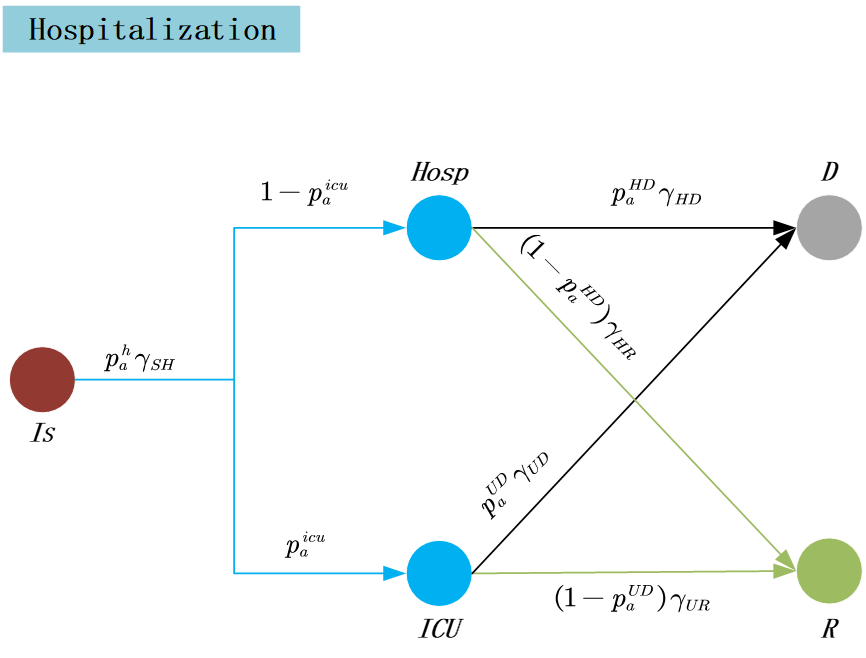
\includegraphics[width=.75\textwidth]{hospital.png}
\caption{上海防控政策的变化和疫情曲线}
\label{hos}
\end{figure}
\par 如图\ref{hos}所示,有症状感染者$I_S$以$p_a^h\gamma_{SH}$的概率会被转运到医院,其中$p_a^h$是有症状感染者中有医院治疗需求的比例,$1/\gamma_{SH}$是有症状感染者被转运至医院的平均天数;转运至医院的人群中,又有占$p_a^{icu}$比例的患者会被转运至ICU;占有两类病床的人群,其死亡率、平均死亡天数、平均康复天数分别为$p_a^{HD}$、$p_a^{UD}$、$1/\gamma_{HD}$、$1/\gamma_{UD}$、$1/\gamma_{HR}$、$1/\gamma_{UR}$。
结合之前对总体状态转移图的分析,有
\begin{equation}
p(D\vert H_a)=p_a^d=p_a^{HD}\frac{1}{\gamma_{HD}}+p_a^{HD}\frac{1}{\gamma_{HD}}
\end{equation}

\begin{equation}
p(R\vert H_a)=1-p_a^d=(1-p_a^{HD})\frac{1}{\gamma_{HR}}+(1-p_a^{UD})\frac{1}{\gamma_{UR}}
\end{equation}
\subsubsection{药物治疗}
抗病毒药物的使用能减轻病情,降低住院率、死亡率。本模型考虑抗病毒药物的效果,将有症状感染者划分为两类:一类是定期使用抗病毒药物的;另外一类不使用抗病毒药物。使用抗病毒药物的患者比例为$p_a^{drug}$。
\begin{figure}[!h]
\centering
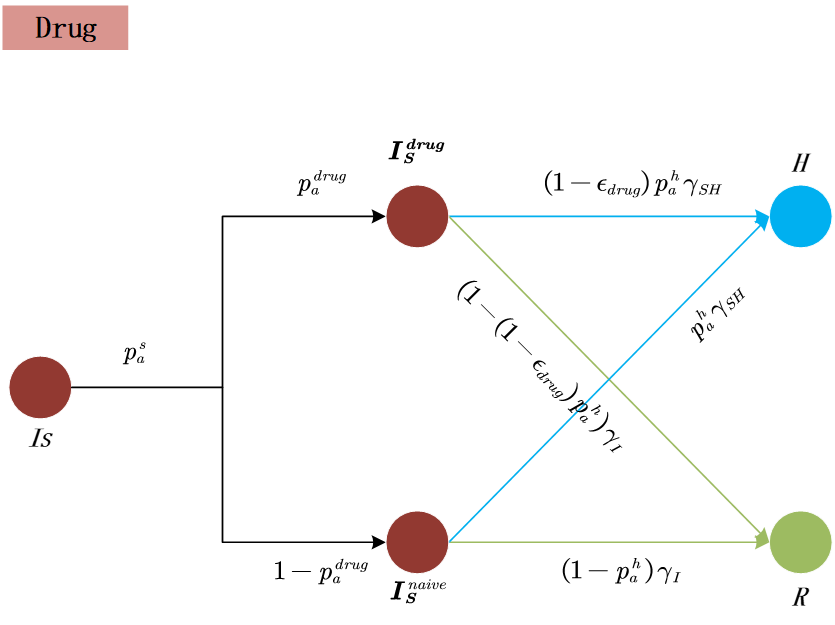
\includegraphics[width=.75\textwidth]{Drug.png}
\caption{药物}
\label{drug}
\end{figure}
\par 如图\ref{drug},$p_a^s$是产生症状的感染者的比例,只有有症状感染者需要接受药物治疗。$p_a^{drug}$是有症状感染者中使用抗病毒药物的比例。药物治疗降低了重症率和死亡率,因此接受药物治疗的患者需要住院的比例更小。$epsilon_{drug}$表示抗病毒药物的效力。使用抗病毒药物的感染者住院和康复的概率分别为
\begin{equation}
p(H\vert I_S^{drug})=(1-\epsilon_{drug})p_a^h\frac{1}{\gamma_{SH}}
\end{equation}
\begin{equation}
p(R\vert I_S^{drug})=(1-(1-\epsilon_{drug})p_a^h)\frac{1}{\gamma_I}
\end{equation}
不使用抗病毒药物的感染者住院和自然康复的概率:
\begin{equation}
p(H\vert I_S^{naive})=p_a^h\frac{1}{\gamma_{SH}}
\end{equation}
\begin{equation}
p(R\vert I_S^{naive})=(1-p_a^h)\frac{1}{\gamma_I}
\end{equation}
\begin{figure}[!h]
\centering
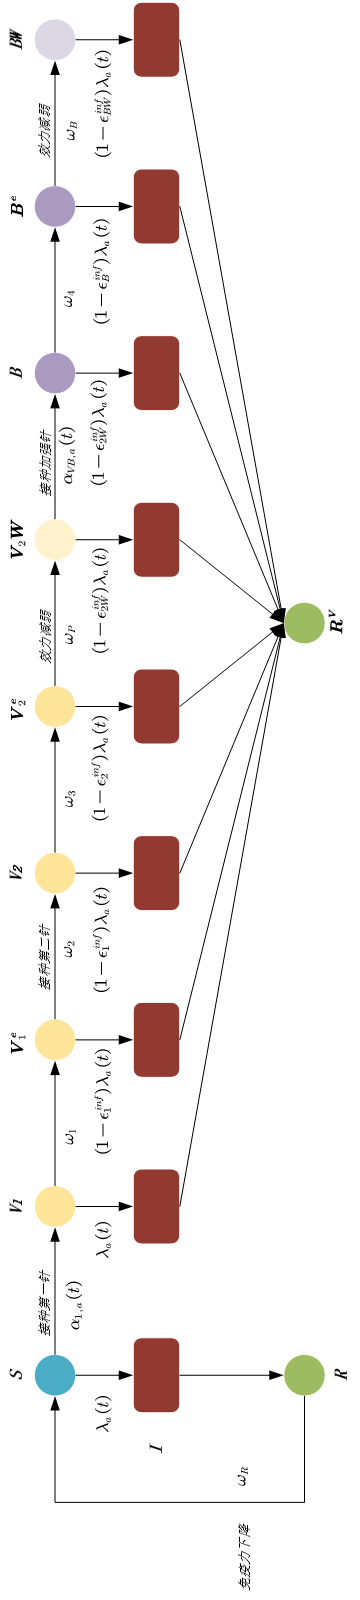
\includegraphics[width=0.36\textwidth]{vaccine.png}
\caption{上海防控政策的变化和疫情曲线}
\label{vac}
\end{figure}
\subsubsection{疫苗}
\par 如图\ref{vac},考虑疫苗效力的变化,将人群分为十二类:
\begin{enumerate}
\item $S,R,I$分别表示未接种过疫苗的易感者、康复者、感染者,未接种过疫苗的康复者对病毒有一定的免疫力,但免疫力会随时间逐渐减弱,最终经$1/\omega_R$时间重新变为易感者;
\item $V_1,V_2,B,$分别表示刚接种过第一针、第二针、加强针疫苗的人群。易感人群接种普通疫苗(第一、二针)的比例为$\alpha _{1}$,接种普通疫苗人群接种加强针的比例为$\alpha_VB$。疫苗生效时间分别是$1/\omega_1,1/\omega_3,1/\omega_4$;
\item $V_1^e,V_2^e,B^e$分别表示接种第一针、第二针、加强针且疫苗生效的人群;
\item $V_2W,BW$表示接种过两剂、三剂疫苗但疫苗效力减退的人群,普通疫苗和加强针效力减退的平均时间为$1/\omega_P,1/\omega_B$;
\item $R^V$表示接种过疫苗并且从感染中恢复的康复者,这类人群对病毒有更高的免疫力
\end{enumerate}
\par 疫苗效力的状态转移与之前所述的状态转移是并行过程。
\subsubsection{时间线分析}

对于美国的疫情数据
对于中国的疫情数据



问题二要求上海在实行初期“精准防控”策略下的疫情发展趋势,并且估算出再生数。
SEIR模型
机器学习方法,时间序列方法
缺乏可解释性

\section{问题求解}
\subsection{数据搜集与预处理}
\par 对于问题一,既然需要拟合参数并进行预测,那么至少需要以下的两组数据:

\begin{enumerate}
    \item 美国COVID-19的相关数据,包括现有病例、治愈数量、死亡人数等。
    \item 中国上海疫情爆发初期的相关数据,用来作为模型的初始数据并进行比对。
\end{enumerate}

\par 有关美国COVID-19的相关数据可以在“Our World In Data”网站上找到,该网站记录了美国2020年3月至今的
所有疫情数据,便于我们用于拟合SIRDT模型的参数。

\par 值得一提的是,由于此次上海疫情的病毒株为传染性极强的奥密克戎变异毒株,所以美国在2020年至2021年的
前期疫情数据并不好直接用于模型参数的拟合,因为普通毒株、$\beta$毒株的基本再生数$R_0$并不相同,所以缺少
一些针对性。

\par 通过相关数据的收集,我们发现从今年一月份开始,美国新冠患者中奥密克戎毒株的份额就已经接近90$\%$了,如
下图所示,这意味着美国今年一月份开始的新冠数据对奥密克戎毒株有较强的针对性。

\begin{figure}[!h]
    \centering
    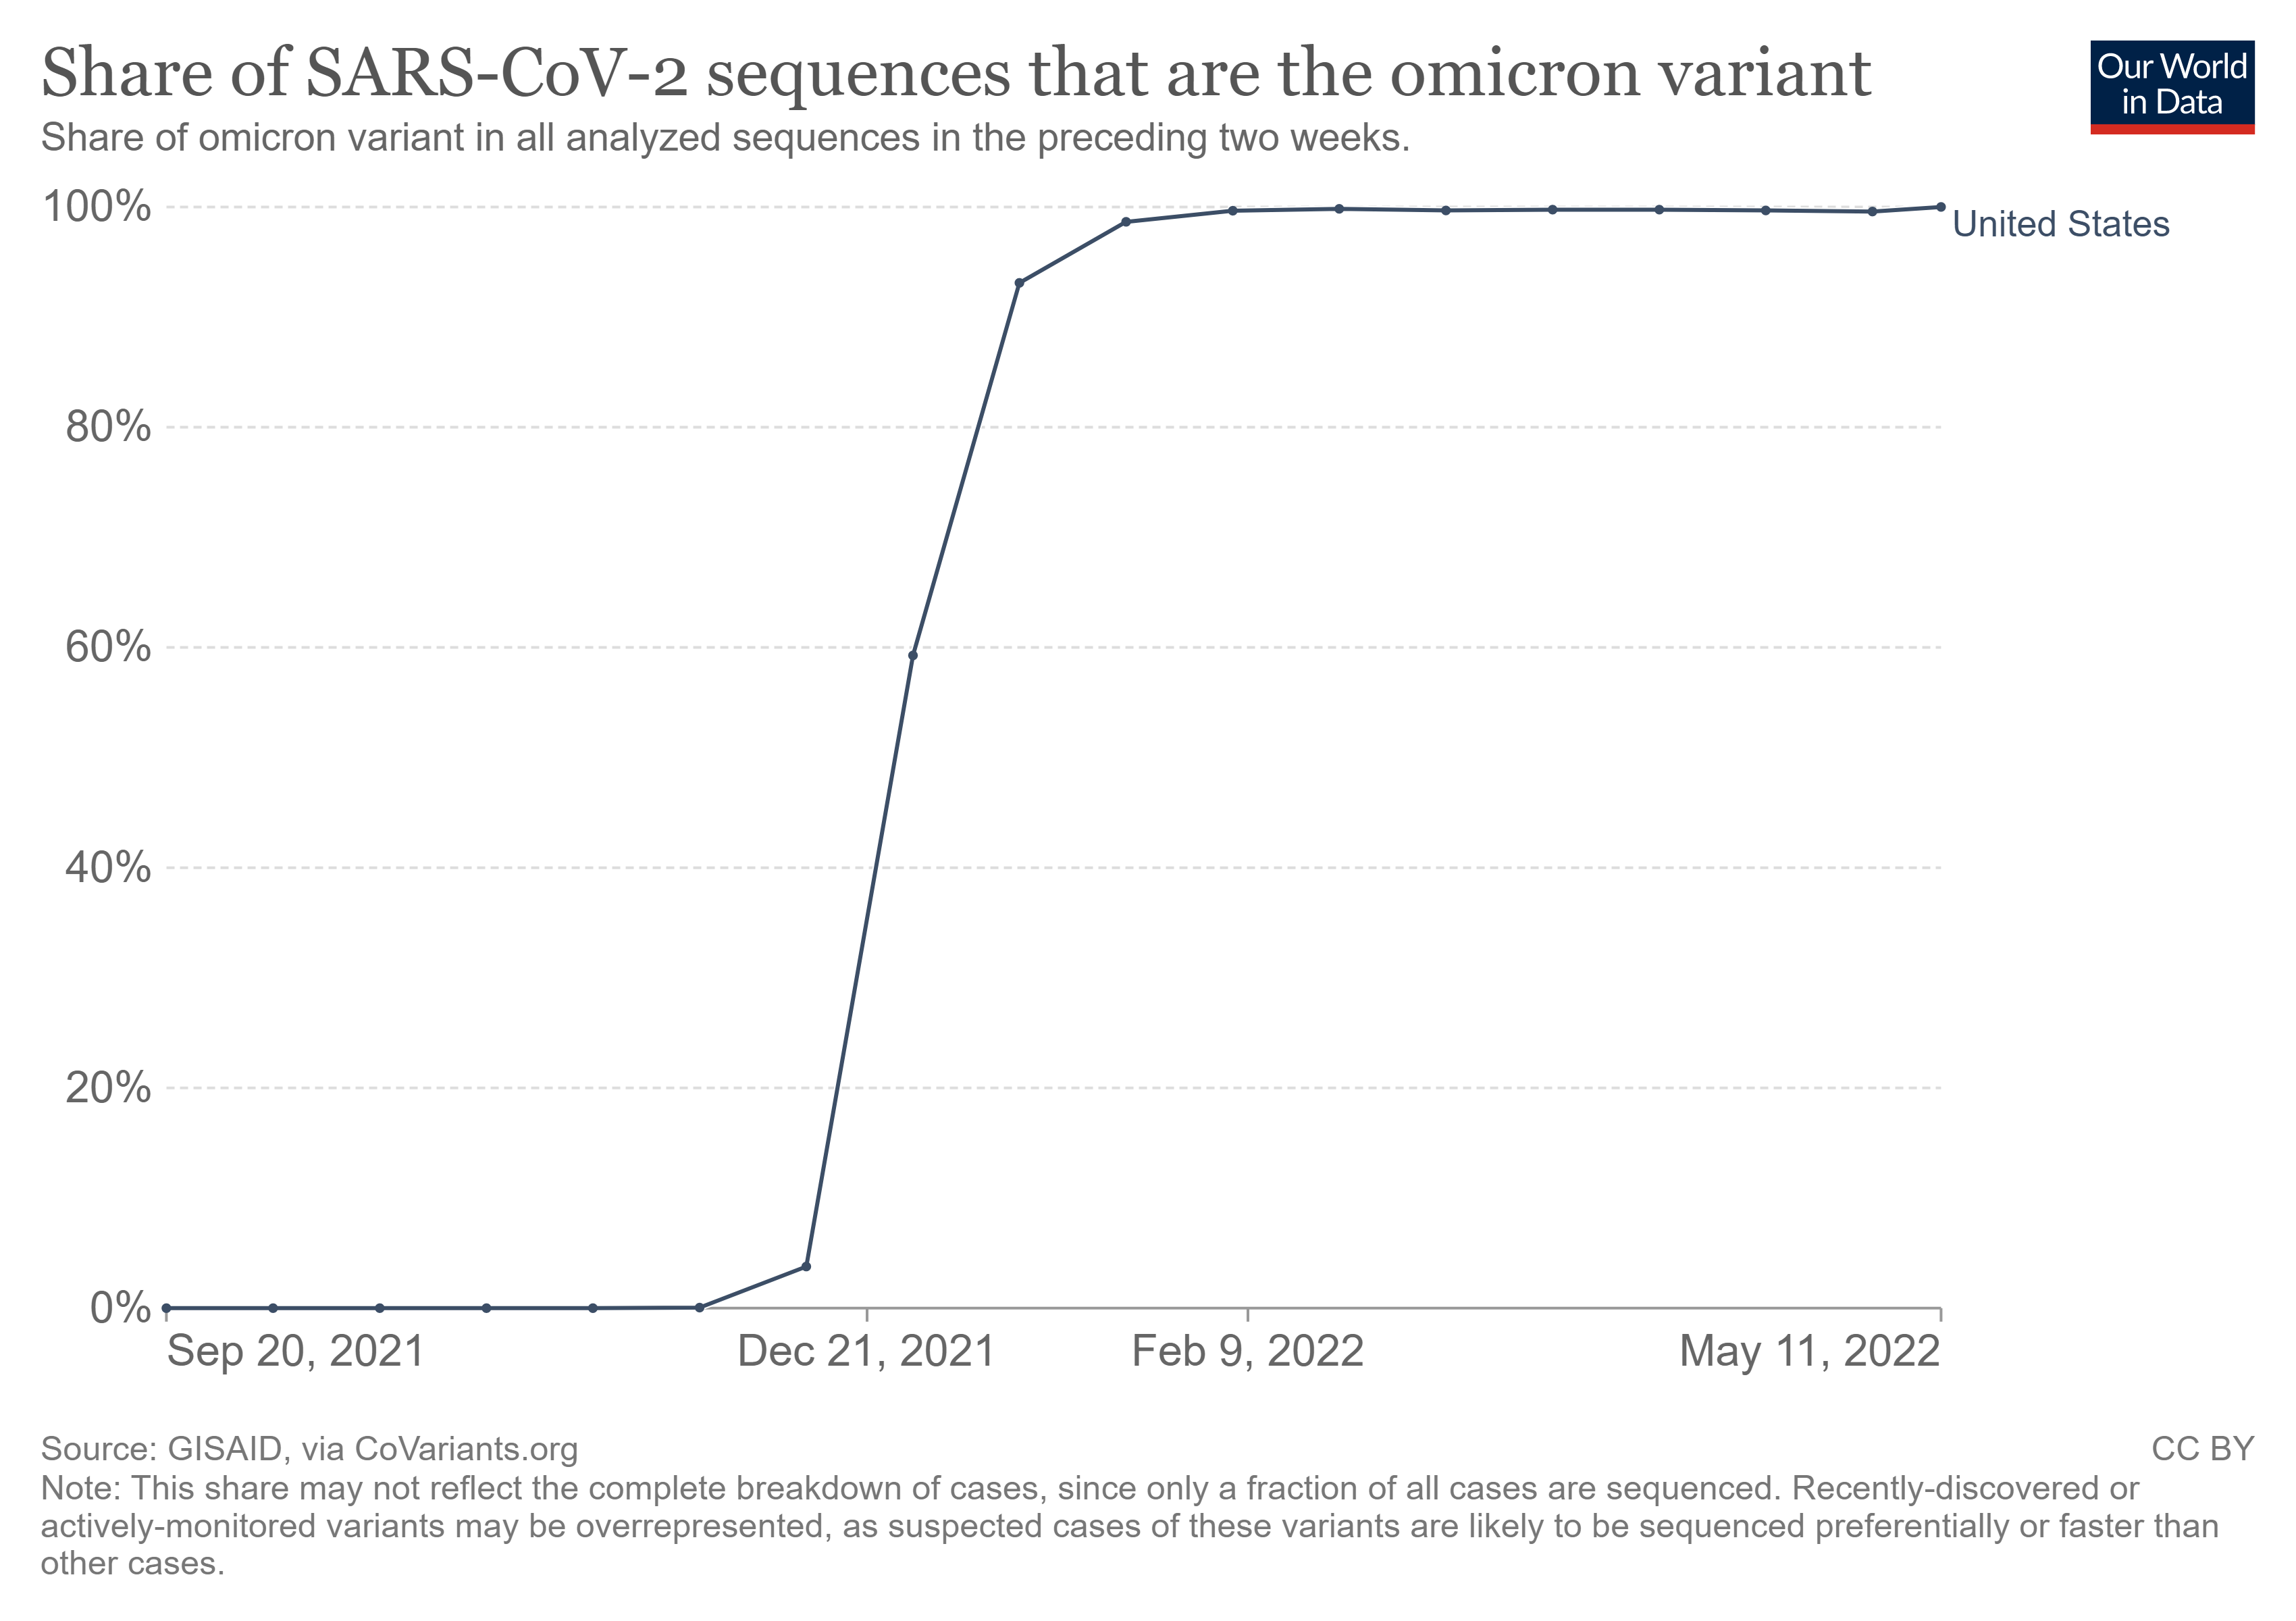
\includegraphics[width=.7\textwidth]{./OmicronVariarntshare.png}
    \caption{奥密克戎毒株所占份额图}
    \label{fig1}
\end{figure}

\par 对于缺失的数据,本文使用了双周期移动平均方法来进行填补,下面将简要介绍双周期移动平均方法,主要公式如下所示:

\begin{equation}
    S_{t}^{'}=\dfrac{x_t+x_{t-1}+\cdots x_{t-N+1}}{N}
\end{equation}

\begin{equation}
    S_{t}^{''}=\dfrac{S_{t}^{'}+S_{t-1}^{'}+\cdots S_{t-N+1}^{'}}{N}
\end{equation}

\begin{equation}
    a_t=2S_{t}^{'}-2S_{t}^{''}
\end{equation}

\begin{equation}
    b_t=\dfrac{2}{N-1}\left( S_{t}^{'}-S_{t}^{''} \right) 
\end{equation}

\begin{equation}
    F_{t+1}=a_t+b_t
\end{equation}

\par 其中式(1)用于计算一次移动平均值, 式(2)用于计算二次移动平均值,式(3)
用于对最新值的初始点进行基本修正,使预测值和实际值之间不存在滞后现象,式(4)表示
移动平均值是对N个点求平均值,这一平均值应落在N个点的中点,式(5)用于计算下一期预测值。
以上海市的治愈数据为例,下面为其对比图:

\begin{figure}[!h]
    \centering
    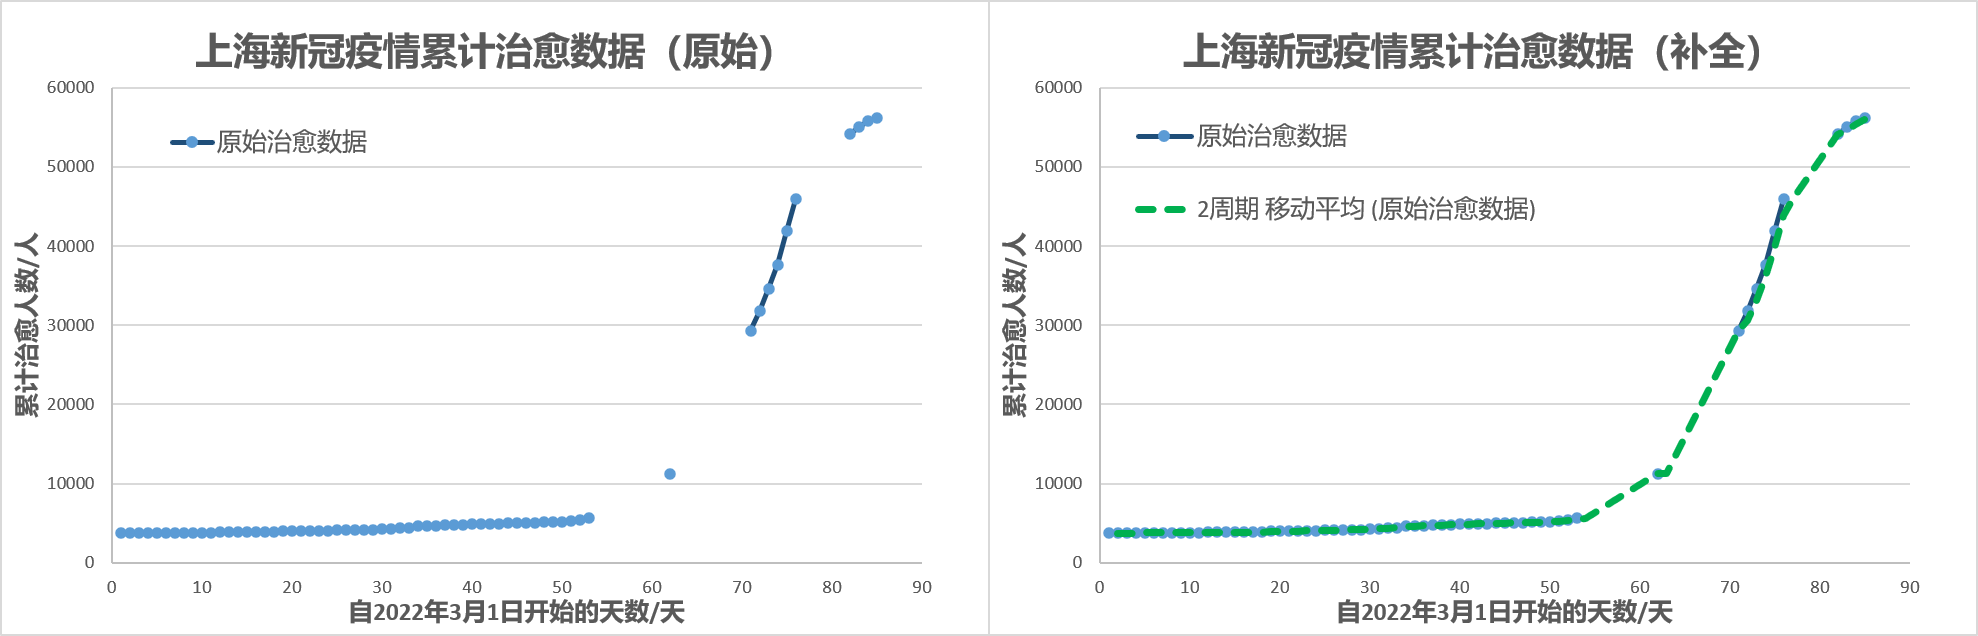
\includegraphics[width=.9\textwidth]{./Cured.png}
    \caption{治愈人数补全前后的对比图}
    \label{fig1}
\end{figure}

\subsection{对问题一的求解}
\subsubsection{模型求解与结论}
\par 为了求解模型,我们首先将SIRDT模型离散化,以天为单位来构建$S$、$I$、$R$的差分方程,具体如下
所示。

\begin{equation} \label{}
    \begin{cases}
        S\left( t+1 \right) =S\left( t \right) -\dfrac{\lambda S\left( t \right) I\left( t \right)}{N\left( t \right)}\\
        I\left( t+1 \right) =I\left( t \right) +\dfrac{\lambda S\left( t \right) I\left( t \right)}{N\left( t \right)}-\mu I\left( t \right)\\
        R\left( t+1 \right) =R\left( t \right) +\mu I_p\left( t \right)\\
        N\left( t \right) =N-D\left( t \right)\\
    \end{cases}
\end{equation}


\par 待求解的目标函数:

\begin{equation} \label{}
    \underset{\lambda ,\mu}{\min}\frac{1}{2}\underset{t=1}{\overset{T}{\varSigma}}\left\| I_r\left( t \right) -I_p\left( t \right) \right\| ^2
\end{equation}

\par 本文使用了BFGS算法来进行参数 $\lambda$ 与 $\mu$ 的拟合。

\par BFGS算法是一种逆秩2拟牛顿法,它由Broyden、Fletcher、Goldfarb、Shanno发明出来,到现在的40多年时间里,
仍然被认为是最好的拟牛顿算法。下面将简述其原理:

\par 其出现的原因就是$H$矩阵求逆非常困难,计算复杂度非常高。BFGS的核心思想就是通过$D_k$
矩阵迭代来代替${H_k}^{-1}$。其逼近公式如下所示:

\begin{equation} \label{}
    D_{k+1}=\left( I-\frac{s_ky_{k}^{T}}{y_{k}^{T}s_k} \right) D_k\left( I-\dfrac{y_ks_{k}^{T}}{y_{k}^{T}s_k} \right) +\dfrac{s_ks_{k}^{T}}{y_{k}^{T}s_k}
\end{equation}

\par 其迭代过程解释如下:

\begin{itemize}
    \item[1)] 其中$I$为单位矩阵,$D_1$的初始值也设置为单位矩阵$I$;
    \item[2)] 首先随机一个$\vec{x}_1$,那么就可以计算的带损失函数在$\vec{x}_1$处的梯度$g_1$;
    \item[3)] $\vec{x}_2=\vec{x}_1-D_1\cdot g_1$,通过此式可以得到$\vec{x}_2$,同时也可以求得$g_2$;
    \item[4)] $s_1=\vec{x}_1-\vec{x}_2$,通过此式可以求得$s_1$;
    \item[5)] $y_1=g_2-g_1$,通过此式可以得到$y_1$;
    \item[6)] 将以上结果带入公式(6)即可得到$D_2$;
    \item[7)] 再用$D_2$来计算$\vec{x}_3$,……,然后不断进行迭代;
    \item[8)] 当$D_n$达到一定的阈值时,停止迭代,此时的$D_n$就可以近似看作${H_k}^{-1}$的值。
\end{itemize}

\par 由于此模型的雅克比矩阵较难求取,所以本文采用了数值梯度的求解方法,在Matlab中使用fmincon函数
来进行了$\lambda$ 与 $\mu$参数的拟合。

\par 根据我们整理的美国奥密克戎毒株自2022年1月1日起的有关数据,拟合出了对应的参数
$\lambda = 0.1345$, $\mu = 0.0768$。并通过以下公式计算出了美国奥密克戎毒株毒株的再生数:

\begin{equation}
    R_t=\dfrac{\lambda}{\mu}
\end{equation}

\par 计算结果为$R_t=1.75$,相比于奥密克戎的基本再生数$R_0=7$已经降低了很多,这说明接种育苗、戴口罩等措施确实
能够有效减少病毒的传播,这相比这与美国官方所公布的1.0左右的有效再生数相差甚远,也间接说明美国
的防疫政策并没有他们所鼓吹的那么出色,在不进行精准防控的情况下,奥密克戎仍有着很强的传染率。
\par 下面是预测数据与真实数据的对比图像:

\begin{figure}[!h]
    \centering
    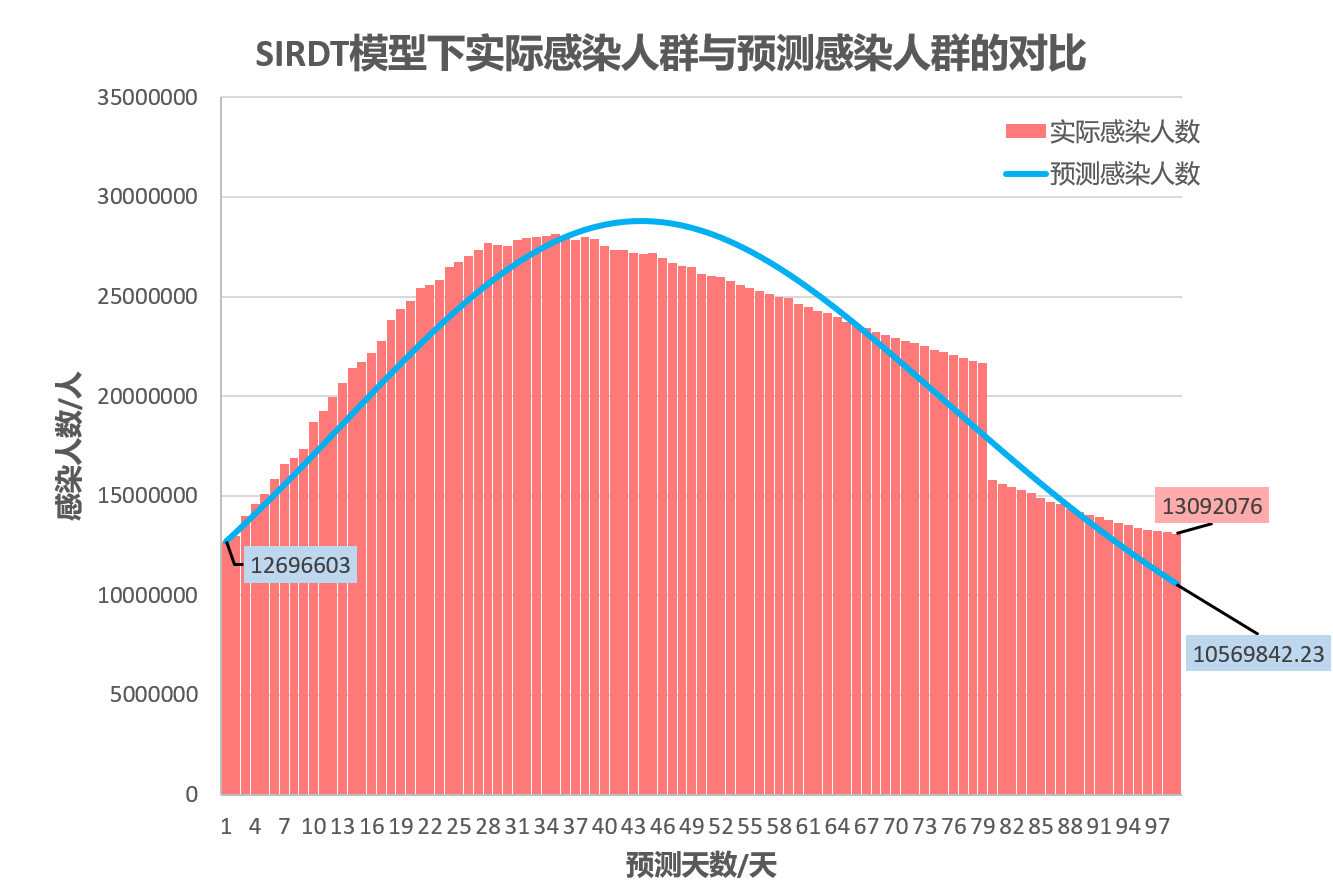
\includegraphics[width=.9\textwidth]{./SIRDT_America.png}
    \caption{SIRDT模型下美国感染人群的预测}
    \label{fig1}
\end{figure}

\par 所取的数据为2022年1月1日后100天内美国的奥密克戎毒株的疫情数据,可以看到,在奥密克戎刚刚出现的时候,美国的
感染人数也是一路飙升,最大现有感染人数最多达到了2700万人,在政府干预后也是慢慢进入到了下降阶段。
\par 之后将计算得到的$\lambda$ 与 $\mu$参数带入经典SIR模型,并以上海3月1日的疫情数据为初始值,即可计算未来两个月
内的发展趋势与累计病例数。其中上海的疫情初始值根据相关数据设置为:

\begin{equation}
    S_0=26315612\text{,}I_0=607\text{,}R_0=3781\text{,}N=26320000
\end{equation}


\par 值得一提的是,为了保证SIR模型的有效性,上海的疫情数据需要做如下的几点处理:
\begin{itemize}
    \item 上海由于本身经历过数次新冠疫情,网络上所获得的疫情数据都是包含前几次疫情的累计确诊与治愈数据,
不能直接拿来进行预测,所以需要进行一些简单的数据处理。在本文中,我们选取3月1日为奥密克戎毒株的起始点,在这一天
的基础上减去之前相应数据,以保证模型能够正确使用。
    \item 但由于相关数据的缺失,上海疫情数据缺少每日的治愈人数,于是为了补全缺失的数据,本文使用了双周期移动
平均方法来补全了缺失的治愈数据。
\end{itemize}


\par 将上述初值与参数带入SIR模型,即可对上海市自3月1日起两个月内的疫情数据进行预测,预测结果如下:

\begin{figure}[!h]
    \centering
    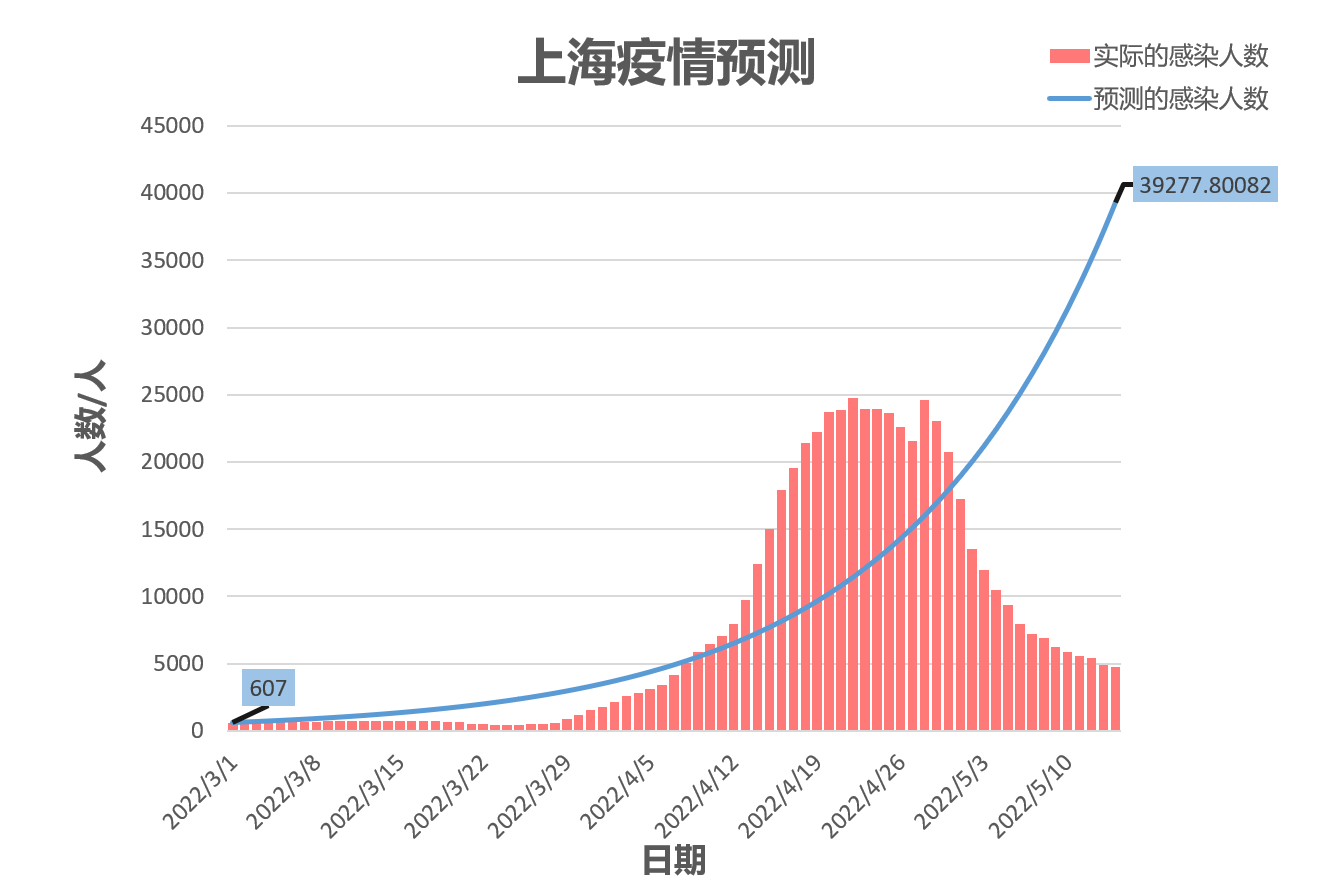
\includegraphics[width=.9\textwidth]{./SH_p.png}
    \caption{上海感染人数预测图}
    \label{fig1}
\end{figure}

\par 当看到绘图出来的结果时,我第一时间其实不太相信,因为预测出来的感染人数增长速率竟然比实际增长的速率要
慢不少,经过分析后,我们发现这样的原因可能是有以下几点:
\begin{itemize}
    \item 虽然表面上上海疫情初期的确诊人数不多,但那是因为上海政府并没有将无症状感染者列入确诊名单,这也就导致
数十倍与确诊人数的无症状感染者没有被考虑到,而无症状感染者的传染能力恰恰更高。
    \item 上海疫情数据很有可能有拖报,瞒报的情况,导致病例数堆积严重,在积累到一定数量后导致数据有爆炸式提升。
    \item 我们使用的是美国2022年1月1日之后一百天的疫情数据来进行参数拟合,但实际上美国的疫情已经。
进入了很长一段时间的平稳期,导致有效再生数$R_t$值偏小,不适用于上海这种爆发初期的情况。
    \item 美国每平方公里人口数为35,上海为32935,人口密度的巨大差距,使得奥密克戎毒株在上海传播更加迅速。
    \item SIRDT、SIR模型还是较为简单,没有考虑到的因素太多,后续需要用更全面的模型来进行预测。
\end{itemize}

\par 由于本模型只是一个简单的模型,没有考虑到感染人数激增对死亡率的影响,但是在实际情况下,上海市的医疗系统肯定会因为过多的病例人数而瘫痪,这会导致患者的死亡率
远远超过1.2$\%$,甚至造成社会的动荡。所以也可以得出结论:如果上海效仿美国的疫情防控措施,秉持以“群体免疫”、
“与病毒共存”的理念,那么在5月14日,现有感染人数将会增加到39000余人。
\par 反过来说,实验结果也说明了疫情爆发后上海市的精准防控策略确实取得了一定的成效,居家隔离等措施让原本飞速增长的感染人数有了明显的下降,将当前的感染人数控制在了4000左右,但也肯定存在
许多的问题,导致感染人数下降的速度较为缓慢。

\par 最后,将计算一下从3月1日至5月10日期间,上海疫情的有效再生数$R_t$的变化情况,以证明政府所采取的封控措施确实有效,
结算结果如下图所示:

\begin{figure}[!h]
    \centering
    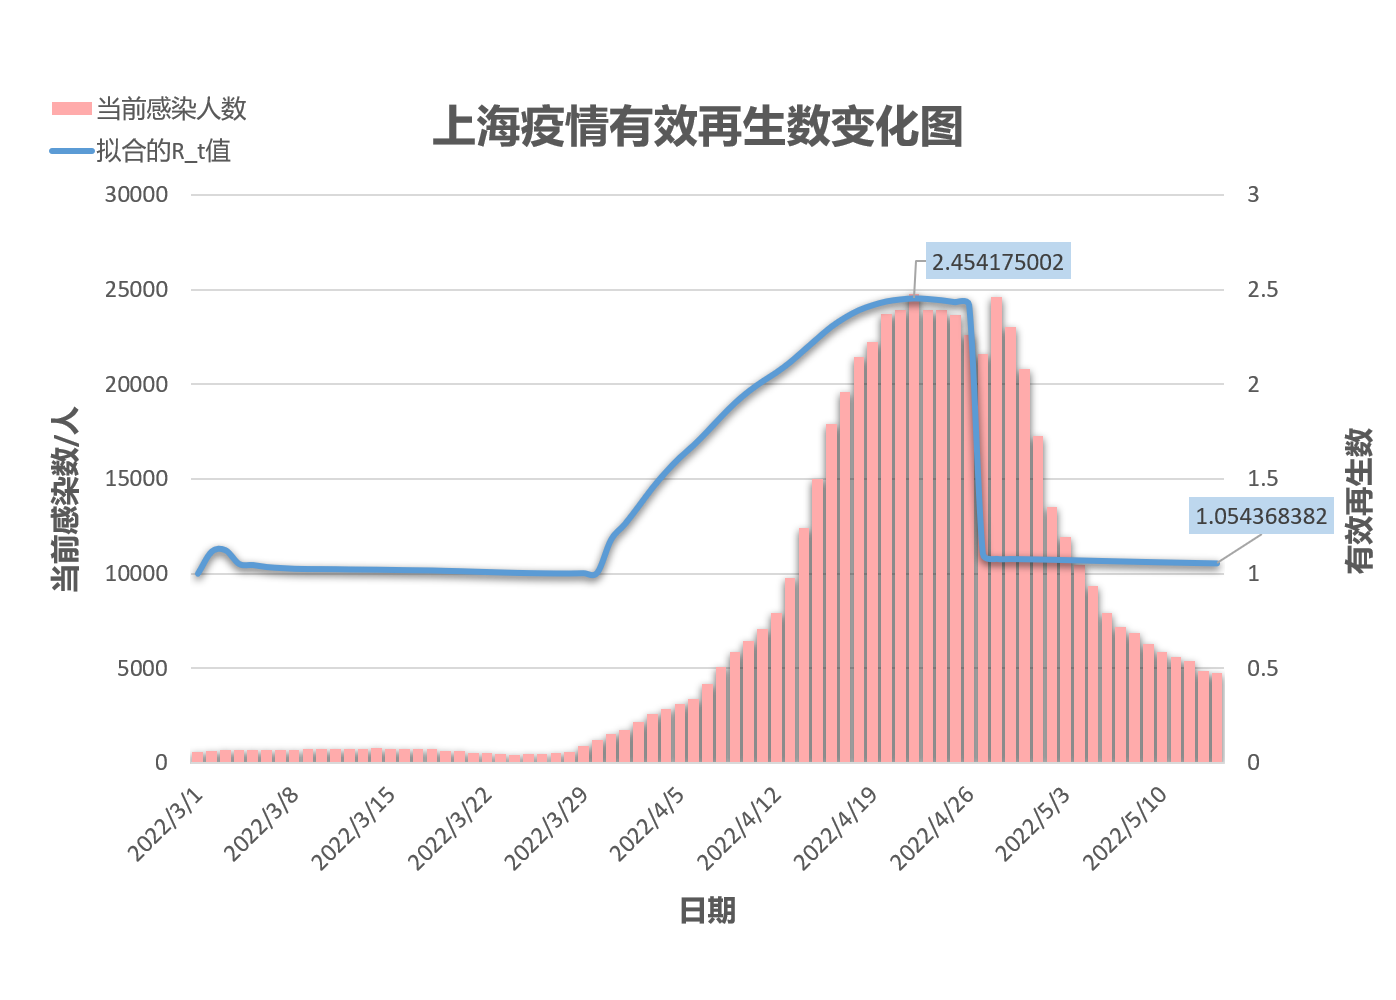
\includegraphics[width=.9\textwidth]{./R_t.png}
    \caption{上海疫情有效再生数变化图}
    \label{fig1}
\end{figure}

\par 由上图可以看出,在大约2022年3月30日之前,$R_t$的值都趋近于1,说明当时的疫情感染人数与治愈人数较为平衡,是可控的,但是在4月1日开始,$R_t$值
开始上升,并在4月19日时达到了最大值2.54,这一段的原因是因为上海开始了大规模核酸与排查,导致之前漏检、瞒报的病例全部暴露了出来,在4月29日左右,$R_t$值又突然
有了断崖式的下跌,重新回到了1附近,使上海疫情形式恢复到了可控状态。


\subsection{对问题二的求解}
精准防控是以最小的经济代价延缓疫情发展,及时发现、隔离感染者和密切接触者,不展开大规模封控,力图将防控影响降低到最小。
\subsubsection{再生数的估计}
\par 对于SLIRS模型,可以求出上海奥密克戎疫情的有效再生数$R_t$,其变化曲线如下图所示:
\begin{figure}[!h]
  \centering
  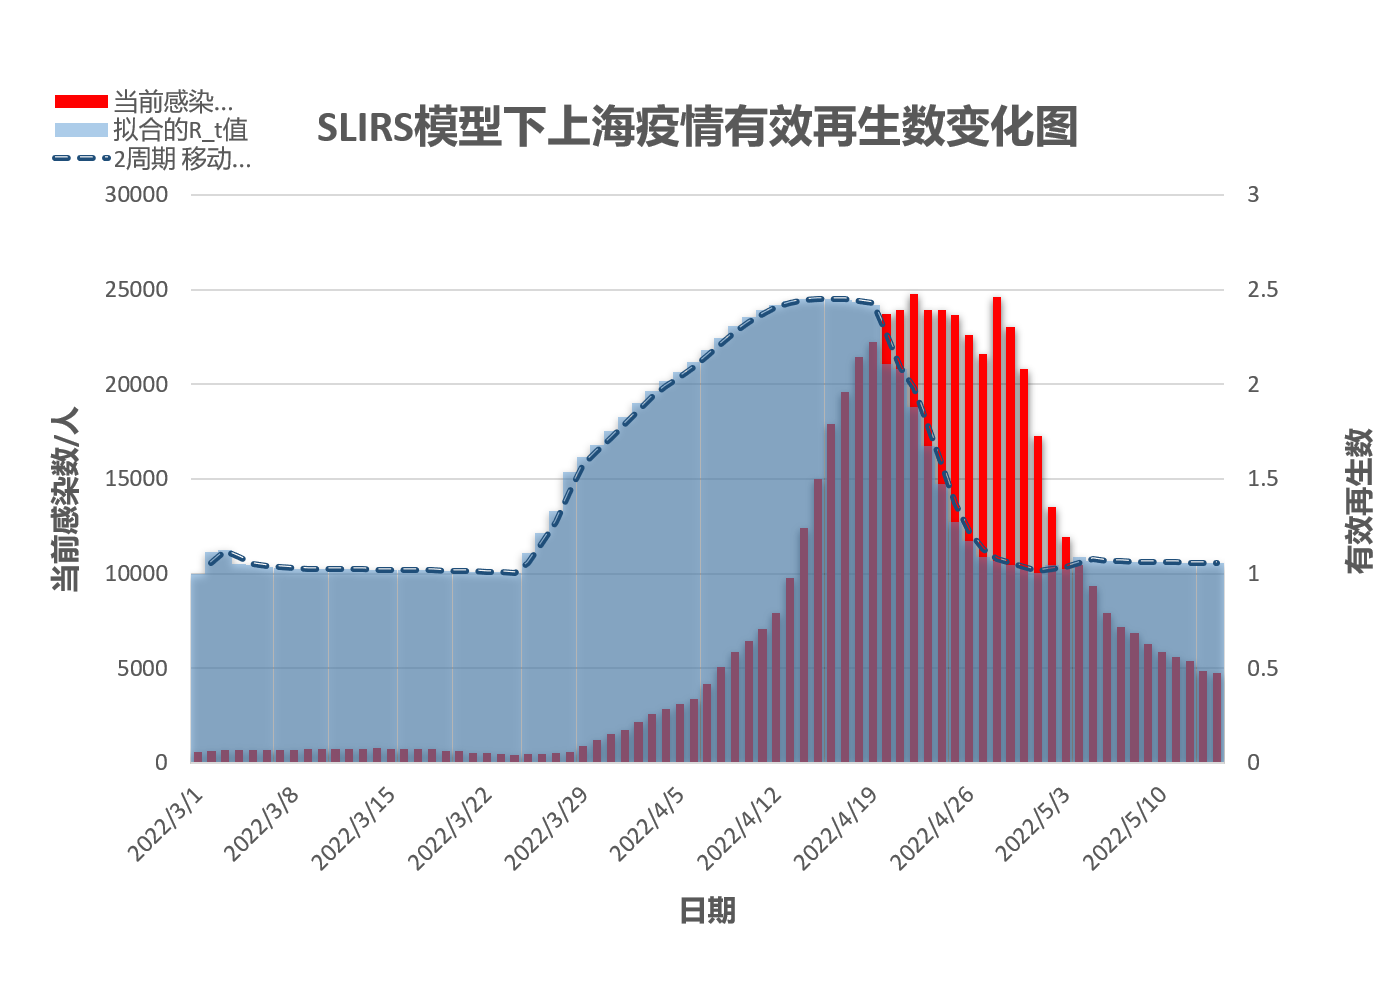
\includegraphics[width=.9\textwidth]{./SLIRS_R_t.png}
  \caption{SLIRS模型下上海疫情有效再生数变化图}
  \label{fig1}
\end{figure}
\par 由图可知,SLIRS所计算的$R_t$与SIR模型下的$R_t$非常相近,但是从时间上有些许提前,数据上更为平滑,最大有效再生数
达到了2.5左右,也比较符合上海疫情的实际。

\subsubsection{模型参数的设置}
\subsubsection{接触矩阵的设置}
上海初期采用精准防控的策略
\subsection{对问题三的求解}
上海加强了管控措施

\section{建议信}
\begin{flushleft}
    尊敬的中共上海市委、上海市人民政府:
\end{flushleft}
\par 你们好
\par 我们是来自南京理工大学的三名研究生,有幸在南京理工大学研究生数学建模竞赛中接触到了上海市疫情预测模型相关的一道题目,通过查阅相关资料、进行模型建立与参数拟合,我们提出了基于XXXXXXXX的新冠肺炎奥密克戎毒株预测模型,并对上海市前期的疫情数据有较好的拟合效果。所以我们将研究结果以书信形式传达,希望能够为上海市的疫情防控奉献我们的一份力量。
\par 自从2022年3月1日上海市此轮本土疫情爆发开始,上海就获取了全国人民的广泛关注。上海作为一个拥有者2500余万常住人口的超大城市,遭受着国际国内多重因素的影响,面临着常态化防控以来最严峻的挑战。
\par 根据我们所构建的预测模型,将为上海市防疫政策提出以下建议:
\par 1. 放开防疫所带来的重症和死亡数量激增可能无法承受。奥密克戎从3月开始不受控制的传播,6个月期间每千人
人口将死亡1.1人,美国的奥密克戎传染期间(2022.1-2022.4),死亡为每千人人口0.57人。中国的数据接近
美国2倍。大面积重症和死亡病例的发生, 不仅导致医疗系统过载,还可能引发经济、社会等多方面问题。
\par 2. 严格防疫措施是缺少特效药及老年疫苗接种率低的无奈之举从最后一个结果可以看到,决定疾病在医
疗系统承载范围内的影响因素,主要是老年疫苗接种率和特效药的普及程度,在这两个条件没有分别接近
100$\%$时,仅有严格防疫措施使$R_t<2$才能保证重症率在可承受范围内,且死亡率与季节性流感相当;但达到
这一标准难度仍较大。一方面,抗病毒药物在不同地区中并不是充分供应,同时也带来巨大的财政负担,老年
疫苗接种率的提升也无法在短期内达到90$\%$以上,因此,在满足这一条件前,严格的防疫措施仍然是降低医
疗负担的唯一的可行策略;
\par 3. 抗病毒药物的有效性较为片面,抗病毒药物在不同研究中的有效性有一定差异,药物的可及性及其所
带来的使用时机的不同,同样会影响有效性,因此,研究中采用的80$\%$和89$\%$都是比较理想的情况;
\par 4. 医疗系统的实际承载能力实际可能更少不论是何种策略施行,当大规模传播发生时,医务人员本身
同样存在感染风险,医疗系统的总容量将显著下降(例如疫情使得英国NHS的医务人员感染而无法工作);
同时医院内部的传染会导致其他疾病的患者发生交叉感染,特别是血液、肿瘤等科室患者本身免疫力较弱,感
染后重症风险更高,且治疗更为复杂;
\par 5. 重症资源缺乏可能导致“只有新冠能进ICU”尽管模拟中,新冠疾病的住院病床采用呼吸专科病床
计算,但ICU资源为全国性资源;在模拟分析中,仅有100患者接受抗病毒药物并老年患者接种加强针后,I
CU资源才满足国内现有情况;但数值仍然占据了大多数ICU病床;如果ICU长期被新冠患者占据,将导致其他
重症患者无法救治,创伤、大手术、抢救等其他重症患者无法治疗;
\par 6. 毒株的变异及地区之间的相互输入没有考虑,研究采用较为固定的传播率和病毒特点,但奥密克戎的
变异株持续发生,传播力和毒力可能发生变化(例如韩国已输入奥密克戎新毒株,传播力进一步增加20$\%$),
因此,即使参照研究中最理想的情况,也无法保证医疗系统能够承载疾病冲击并降低重症和死亡几率。因此,
从科学角度来说,现有策略是较为可行、风险可控的防疫政策;基于现有政策,进一步平衡经济、社会因素,
提升社会保障是更加科学的防疫办法。
\par 上海市人口基数大,防疫压力大、难度高,我们都能够理解,也相信所有中国人民、上海人民也都能理解。疫情当头,现在不是指责与推卸责任的时候,而是正面解决问题的关键时刻,希望我们的政府公职人员能够拿出共产党人的责任与担当,我们一起打赢上海市的疫情防控阻击战。也希望如国家卫健委新冠肺炎疫情应对处置工作领导小组专家组组长梁万年所说的,在执行防疫政策的过程中,做到真正“有温度”的防疫,发扬我们社会主义国家的人文关怀,而不
是一味只看规章制度,不近人情。
\par 我们曾去过上海,去看过绚丽的霓虹灯下东方明珠的辉煌,黄浦江上耀眼的光芒中蕴藏着一种近代的沧桑。弄堂中老上海人将油灯点亮,星星点点照亮长廊,临街的商铺里是闪亮的衣裳,美丽的上海让我们如此沉醉,虽许久不见,但仍想念那人流如潮、车水马龙的繁华与奔忙。
\\
\par 愿:
\begin{flushleft}
    上海一切安好,所有上海人民早日走出疫情阴霾!
\end{flushleft}
\begin{flushright}
    几名持续关注上海疫情的南理工学子
    \par 2022年 5月 16日
\end{flushright}

\section{模型的评价}
\subsection{模型的优点}
\par 对于用来解答第一问的SIRDT与SIR模型,其优点主要有以下方面:
\begin{enumerate}
  \item 模型简介明了,各个数据非常直观,参数也都具有实际意义,方便对疫情发展情况进行简单快速的了解;
  \item 操作简单,不需要复杂的函数、代码,大大减少了运行时间。
  传播的有效手段;
  \end{enumerate}
\par 对于用来解答第二问、第三问的SLIRS模型,其优点主要体现在以下方面:

\subsection{模型的缺点}
\par 对于用来解答第一问的SIRDT与SIR模型,其缺点主要体现过于理想化,没有能够完全
考虑奥密克戎缺乏特异性表现、鉴别诊断难度大、传播更加隐匿等特性,具体体现在以下方面:
\begin{enumerate}
  \item 模型对人群的分类不够细致,只考虑了$S$、$I$、$R$、$D$几个基本人群类别,而且没有考虑奥密克戎对不
  同年龄段人群的传染性的不同;
  \item 没有考虑隔离、疫苗等的因素对奥密克戎的影响,没有一个量化的参数与指标,而现实中对疑似病人的隔离是控制疫情
  传播的有效手段;
  \item 模型没有引入反馈机制,在预测过程中,单纯依据已有数据预测未来较长一段时间的数据,必然会使准确度降低。此外,微分方程组求解较为困难,且
  对初值比较敏感,这对模型的稳健性是一个很大的影响。
  \end{enumerate}
\par 对于用来解答第二问、第三问的SLIRS模型,其缺点主要体现在以下方面:

\section{参考文献}
%参考文献
\begin{thebibliography}{1.2}%宽度9
\setlength{\itemsep}{-2mm}
 \bibitem{bib:one} 
 韩中庚. 数学建模方法及其应用[M]. 高等教育出版社, 2005.
 \bibitem{bib:two}
 韩中庚. 数学建模方法及其应用[M]. 高等教育出版社, 2005.
  \bibitem{bib:two}
 韩中庚. 数学建模方法及其应用[M]. 高等教育出版社, 2005.
\end{thebibliography}

\bibliographystyle{plain}
\bibliography{ref}

\newpage
%附录
\appendix
\section{程序代码}
%设置不同语言即可。
\begin{lstlisting}[language=Matlab] 
% 主函数

n_sim = "10" ;    % simulation times, max 200
t_simulate = "180" ;    % time for simulation in days
input_folder = "./Model_Omicron_China/INPUT_SH" ;    % input folder for parameters
t_epistart = "457" ;    % start date of epidemic, "457" indicates "2022-03-01"
n_initialinfectors = "20" ;    % initial infectors introduced
R0 = "3.9" ;    % reproduction number
booster_target = "18p" ;    % target booster age-group
booster_regimen = "Inactivated" ;    % booster vaccination type
booster_supply = "5000000" ;    % booster supply since epidemic
booster_acceptance = "0.9" ;    % rate for people accept to have booster shot
drug_uptake = "0" ;    % proportion of drug uptake
drug_effect = "0.8" ;    % effectiveness for drug
cm = "baseline" ;    % contact matrix setting
sus_type = "hetero" ;    % susceptibility setting
kappa = "1" ;    % infectivity for asymptomatic cases
GT = "L" ;    % rate for transmission setting, include generation time
RNG_seed = "1" ;    % seed for random number generator, must be an int
VE_setting = "OPT_ONE" ;    % VE setting, see table above for "INPUT_CN"
limits4elderly = "YES" ;    % limits for vaccination for elderly
prob_folder = "SA" ;    % folder name for probability parameter
save_prefix = "./Model_Omicron_China/OUTPUT/OPT=school_close_SH" ;    % save path prefix
asymp_scale = "0.15" ;    % adjusted ratio for asymptomatic cases
delta_infection = "0" ;    % proportion for prior delta_infection
cmd = '/Users/yibeibankaishui/Desktop/MathModeling-2022-NJUST-BLM...
/codes/Model_Omicron_China/SEIRS';

str = [cmd n_sim, t_simulate, input_folder, t_epistart, n_initialinfectors, R0, booster_target, booster_regimen,... 
    booster_supply, booster_acceptance, drug_uptake, drug_effect, cm, sus_type, ...
    kappa, GT, RNG_seed, VE_setting, limits4elderly, prob_folder, save_prefix, ...
    asymp_scale, delta_infection];

command = join(str);

[status,cmdout] = system(command);

 \end{lstlisting}
 
 
 \begin{lstlisting}[language=C] 
% 主函数
#include "head.h"

int main(int argc, char *argv[])
{
  char help[] = "PARAMTERS NOT ADEQUATE!!!";
  if (argc < 23)
  {
    fprintf(stderr, "%s\n", help);
    exit(1);
  }

  // SET ALL INPUT
  int SIM_MAX = atoi(argv[1]);
  int T_EPIDURATION = atoi(argv[2]);
  char *CITY_SELECTED = argv[3];

  int T_EPISTART = atoi(argv[4]);
  int N_initial_I = atoi(argv[5]);
  double BETA = atof(argv[6]);
  char *STRATEGY4BOOST = argv[7];
  char path_STRATEGY4BOOST[100];
  sprintf(path_STRATEGY4BOOST, "%s/VAC/VB2%s", CITY_SELECTED, STRATEGY4BOOST);
  char *TYPE4BOOST = argv[8];
  int BOOST_SUPPLY = atoi(argv[9]);
  double BOOST_COVERAGE = atof(argv[10]);
  double p_DRUG = atof(argv[11]);
  double rate4DRUG = atof(argv[12]);
  char *TYPE4CM = argv[13];
  char path_CM[100], path_CM4beta[100];
  char *TYPE4SUS = argv[14];
  char path_TYPE4SUS[100];
  sprintf(path_TYPE4SUS, "%s/POP/%s_sus", CITY_SELECTED, TYPE4SUS);
  double Kappa = atof(argv[15]);
  char *TYPE4GAMMA = argv[16];
  char path_TYPE4GAMMA[100];
  sprintf(path_TYPE4GAMMA, "%s/Gamma_%s", CITY_SELECTED, TYPE4GAMMA);
  int RNG_SEED = atoi(argv[17]);
  char *TYPE4VE = argv[18];
  char path_VE[100];
  sprintf(path_VE, "%s/VE/VE_%s_%s", CITY_SELECTED, TYPE4VE, TYPE4BOOST);
  char *WHE_60 = argv[19];
  char path_CONTRA[100];
  sprintf(path_CONTRA, "%s/POP/contraindication_%s", CITY_SELECTED, WHE_60);
  char *TYPE4OUTCOME = argv[20];
  char path_TYPE4OUTCOME[100];
  sprintf(path_TYPE4OUTCOME, "%s/PROB_%s/", CITY_SELECTED, TYPE4OUTCOME);
  char *path_SAVE = argv[21];
  double p_scale4symp = atof(argv[22]);
  int whe_delta = atoi(argv[23]);

  // TRANSMISSION RELATED PARAMETERS
  int T_STEP = 1, N[N_AGE], AGE_selected, whe_CS;
  int num_vac_trans = 0;
  double Beta, I_COUNT;

  // DECLARE ALL COMPARTMENTS
  STATE_SEIR STATE_S, STATE_V1, STATE_V1E, STATE_V1W, STATE_V2, STATE_V2E, STATE_V2W;
  STATE_SEIR STATE_V3, STATE_V3E, STATE_V3W, STATE_R, STATE_RDelta;

  // GENERATE ALL SAVE
  SAVE save_STATE_S, save_STATE_V1, save_STATE_V1E, save_STATE_V1W, save_STATE_V2, save_STATE_V2E, save_STATE_V2W;
  SAVE save_STATE_V3, save_STATE_V3E, save_STATE_V3W, save_STATE_R, save_STATE_RDelta;
  SAVE save_NEW_S, save_NEW_V1, save_NEW_V1E, save_NEW_V1W, save_NEW_V2, save_NEW_V2E, save_NEW_V2W;
  SAVE save_NEW_V3, save_NEW_V3E, save_NEW_V3W, save_NEW_R, save_NEW_RDelta;

  // VACCINE RELATED INPUT
  int VP_strategy[N_AGE][4], VB_strategy[N_AGE][1];
  int VP_index, VB_index, VP_dose, VB_dose, DOSE_REMAINED;
  int INPUT_VP_dose[T_EPISTART + T_EPIDURATION], INPUT_VB_dose[T_EPISTART + T_EPIDURATION];
  int V1_admin[N_AGE], V2_admin[N_AGE], VB_admin[N_AGE];

  char path_VP[100], path_VB[100], path_STRATEGY4VP[100];
  sprintf(path_VP, "%s/VAC/VP_ts", CITY_SELECTED);
  sprintf(path_VB, "%s/VAC/VB_ts", CITY_SELECTED);
  sprintf(path_STRATEGY4VP, "%s/VAC/VP_strategy", CITY_SELECTED);
  FUNC_read_col_int(path_VP, T_EPISTART + T_EPIDURATION, INPUT_VP_dose);
  FUNC_read_col_int(path_VB, T_EPISTART + T_EPIDURATION, INPUT_VB_dose);
  FUNC_read_matrix_int(path_STRATEGY4VP, N_AGE, 4, VP_strategy);
  FUNC_read_matrix_int(path_STRATEGY4BOOST, N_AGE, 1, VB_strategy);

  // POPULATION RELATED INPUT
  double RATE_contra[N_AGE], RATE_sus[SIM_MAX][N_AGE], CM[N_AGE][N_AGE], CM4Beta[N_AGE][N_AGE], Gamma[7];
  double Lambda[N_AGE], p_foi[N_AGE], p_V1[N_AGE], p_V1E[N_AGE], p_V1W[N_AGE];
  double p_V2[N_AGE], p_V2E[N_AGE], p_V2W[N_AGE];
  double p_V3[N_AGE], p_V3E[N_AGE], p_V3W[N_AGE];
  double p_R[N_AGE], p_RDelta[N_AGE];

  char path_N[100];
  sprintf(path_N, "%s/POP/population", CITY_SELECTED);
  FUNC_read_col_int(path_N, N_AGE, N);
  FUNC_read_col_double(path_CONTRA, N_AGE, RATE_contra);
  FUNC_read_matrix_double(path_TYPE4SUS, SIM_MAX, N_AGE, RATE_sus);

  // DISEASE PARAMETERS INPUT
  FUNC_read_col_double(path_TYPE4GAMMA, 7, Gamma);
  GAMMA day_Gamma = {Gamma[0] / (double)T_STEP, Gamma[1] / (double)T_STEP, Gamma[2] / (double)T_STEP,
                     Gamma[3] / (double)T_STEP, Gamma[4] / (double)T_STEP, Gamma[5] / (double)T_STEP,
                     Gamma[6] / (double)T_STEP};
  GAMMA p_Gamma = {1.0 - exp(-Gamma[0] / (double)T_STEP), 1.0 - exp(-Gamma[1] / (double)T_STEP),
                   1.0 - exp(-Gamma[2] / (double)T_STEP), 1.0 - exp(-Gamma[3] / (double)T_STEP),
                   1.0 - exp(-Gamma[4] / (double)T_STEP), 1.0 - exp(-Gamma[5] / (double)T_STEP),
                   1.0 - exp(-Gamma[6] / (double)T_STEP)};

  PROB_PROGRESS p_OUTCOME;
  double p_symp[N_AGE], p_hosp[N_AGE], p_icu[N_AGE], p_death_icu[N_AGE], p_death_hos[N_AGE];
  char path_SYMP[100], path_HOSP[100], path_ICU[100], path_DEATH_ICU[100], path_DEATH_HOSP[100];
  strcpy(path_SYMP, path_TYPE4OUTCOME);
  strcat(path_SYMP, "p_symp");
  strcpy(path_HOSP, path_TYPE4OUTCOME);
  strcat(path_HOSP, "p_hosp");
  strcpy(path_ICU, path_TYPE4OUTCOME);
  strcat(path_ICU, "p_icu");
  strcpy(path_DEATH_ICU, path_TYPE4OUTCOME);
  strcat(path_DEATH_ICU, "p_death_icu");
  strcpy(path_DEATH_HOSP, path_TYPE4OUTCOME);
  strcat(path_DEATH_HOSP, "p_death_h");
  FUNC_read_col_double(path_SYMP, N_AGE, p_symp);
  FUNC_read_col_double(path_HOSP, N_AGE, p_hosp);
  FUNC_read_col_double(path_ICU, N_AGE, p_icu);
  FUNC_read_col_double(path_DEATH_ICU, N_AGE, p_death_icu);
  FUNC_read_col_double(path_DEATH_HOSP, N_AGE, p_death_hos);

  for (int i = 0; i < N_AGE; i++)
  {
    p_OUTCOME.Symp[i] = p_scale4symp * p_symp[i];
    p_OUTCOME.Hosp[i] = p_hosp[i];
    p_OUTCOME.ICU[i] = p_icu[i];
    p_OUTCOME.Death_ICU[i] = p_death_icu[i];
    p_OUTCOME.Death_HOS[i] = p_death_hos[i];
    if (i <= 1)
    {
      p_OUTCOME.Drug[i] = 0.0;
    }
    else
    {
      p_OUTCOME.Drug[i] = p_DRUG;
    }
  }

  // VE INPUT
  VE VE_4_S, VE_4_V1, VE_4_V1E, VE_4_V1W, VE_4_V2, VE_4_V2E, VE_4_V2W;
  VE VE_4_V3, VE_4_V3E, VE_4_V3W, VE_4_R, VE_4_RDelta;
  double TMP_VE[7][12];
  FUNC_read_matrix_double(path_VE, 7, 12, TMP_VE);
  FUNC_read_VE(12, 0, TMP_VE, &VE_4_S);
  FUNC_read_VE(12, 1, TMP_VE, &VE_4_V1);
  FUNC_read_VE(12, 2, TMP_VE, &VE_4_V1E);
  FUNC_read_VE(12, 3, TMP_VE, &VE_4_V1W);
  FUNC_read_VE(12, 4, TMP_VE, &VE_4_V2);
  FUNC_read_VE(12, 5, TMP_VE, &VE_4_V2E);
  FUNC_read_VE(12, 6, TMP_VE, &VE_4_V2W);
  FUNC_read_VE(12, 7, TMP_VE, &VE_4_V3);
  FUNC_read_VE(12, 8, TMP_VE, &VE_4_V3E);
  FUNC_read_VE(12, 9, TMP_VE, &VE_4_V3W);
  FUNC_read_VE(12, 10, TMP_VE, &VE_4_R);
  FUNC_read_VE(12, 11, TMP_VE, &VE_4_RDelta);

  // DELTA COMPARMENT
  int N_Delta[123][N_AGE], AGE_SUM, AGE_EACH[8];
  char path_Delta[500];
  sprintf(path_Delta, "%s/Delta_inf", CITY_SELECTED);
  FUNC_read_matrix_int(path_Delta, 123, N_AGE, N_Delta);

  // INITIALIZE GSL RANDOM GENERATOR
  gsl_rng *RNG;
  RNG = gsl_rng_alloc(gsl_rng_default);
  gsl_rng_set(RNG, RNG_SEED);

  // SAVE PATH AND DECLARATION
  char path_save1[500], path_save2[500], path_save3[500];
  sprintf(path_save1, "%s+new_I_Is_H_ICU_D_byS-V1-V2-V3-V1E-V2E-V3E-V1W-V2W-V3W-R-RDelta.txt", path_SAVE);
  sprintf(path_save2, "%s+state_S_Is_H_ICU_D_byS-V1-V2-V3-V1E-V2E-V3E-V1W-V2W-V3W-R-RDelta.txt", path_SAVE);
  sprintf(path_save3, "%s+vac_V1_V2_VB.txt", path_SAVE);

  FILE *f_save1;
  f_save1 = fopen(path_save1, "w");
  FILE *f_save2;
  f_save2 = fopen(path_save2, "w");
  FILE *f_save3;
  f_save3 = fopen(path_save3, "w");

  // SIM START
  for (int sim = 0; sim < SIM_MAX; sim++)
  {
    printf("SIM-%+3d: ", sim);

    sprintf(path_CM, "%s/CM/%s/cm_%d", CITY_SELECTED, TYPE4CM, sim);
    sprintf(path_CM4beta, "%s/CM/baseline/cm_%d", CITY_SELECTED, sim);
    FUNC_read_matrix_double(path_CM, N_AGE, N_AGE, CM);
    FUNC_read_matrix_double(path_CM4beta, N_AGE, N_AGE, CM4Beta);

    // INITIALIZE COMPARTMENT WITH 0
    for (int i = 0; i < N_AGE; i++)
    {
      V1_admin[i] = 0;
      V2_admin[i] = 0;
      VB_admin[i] = 0;
      FUNC_zero_SEIR(i, &STATE_S);
      FUNC_zero_SEIR(i, &STATE_V1);
      FUNC_zero_SEIR(i, &STATE_V1E);
      FUNC_zero_SEIR(i, &STATE_V1W);
      FUNC_zero_SEIR(i, &STATE_V2);
      FUNC_zero_SEIR(i, &STATE_V2E);
      FUNC_zero_SEIR(i, &STATE_V2W);
      FUNC_zero_SEIR(i, &STATE_V3);
      FUNC_zero_SEIR(i, &STATE_V3E);
      FUNC_zero_SEIR(i, &STATE_V3W);
      FUNC_zero_SEIR(i, &STATE_R);
      FUNC_zero_SEIR(i, &STATE_RDelta);

      FUNC_zero_SAVE(i, &save_STATE_S);
      FUNC_zero_SAVE(i, &save_STATE_V1);
      FUNC_zero_SAVE(i, &save_STATE_V1E);
      FUNC_zero_SAVE(i, &save_STATE_V1W);
      FUNC_zero_SAVE(i, &save_STATE_V2);
      FUNC_zero_SAVE(i, &save_STATE_V2E);
      FUNC_zero_SAVE(i, &save_STATE_V2W);
      FUNC_zero_SAVE(i, &save_STATE_V3);
      FUNC_zero_SAVE(i, &save_STATE_V3E);
      FUNC_zero_SAVE(i, &save_STATE_V3W);
      FUNC_zero_SAVE(i, &save_STATE_R);
      FUNC_zero_SAVE(i, &save_STATE_RDelta);

      FUNC_zero_SAVE(i, &save_NEW_S);
      FUNC_zero_SAVE(i, &save_NEW_V1);
      FUNC_zero_SAVE(i, &save_NEW_V1E);
      FUNC_zero_SAVE(i, &save_NEW_V1W);
      FUNC_zero_SAVE(i, &save_NEW_V2);
      FUNC_zero_SAVE(i, &save_NEW_V2E);
      FUNC_zero_SAVE(i, &save_NEW_V2W);
      FUNC_zero_SAVE(i, &save_NEW_V3);
      FUNC_zero_SAVE(i, &save_NEW_V3E);
      FUNC_zero_SAVE(i, &save_NEW_V3W);
      FUNC_zero_SAVE(i, &save_NEW_R);
      FUNC_zero_SAVE(i, &save_NEW_RDelta);

      STATE_S.C[i] = (int)(RATE_contra[i] * (double)N[i] + 0.5);
      STATE_S.S[i] = N[i] - STATE_S.C[i];

      for (int j = 0; j < N_AGE; j++)
      {
        CM[i][j] = CM[i][j] * RATE_sus[sim][i];
        CM4Beta[i][j] = CM4Beta[i][j] * RATE_sus[sim][i];
        CM4Beta[i][j] = ((Kappa * (1.0 - p_OUTCOME.Symp[j])) / day_Gamma.I2R + p_OUTCOME.Symp[j] / (day_Gamma.I2R * (1.0 - p_OUTCOME.Hosp[j]) + day_Gamma.Is2H * p_OUTCOME.Hosp[j])) * CM4Beta[i][j] * N[i] / N[j];
      }
    }

    Beta = BETA / FUNC_NGM(N_AGE, CM4Beta);

    VP_index = VB_index = 0;

    // main loop
    for (int t = 0; t < (T_EPISTART + T_EPIDURATION) * T_STEP; t++)
    {
      fprintf(f_save1, "%d %d", sim, t);
      fprintf(f_save2, "%d %d", sim, t);
      fprintf(f_save3, "%d %d", sim, t);

      // ALLOCATE INITIAL INFECTORS
      if (t == (T_EPISTART - 1) * T_STEP)
      {
        for (int i = 0; i < N_initial_I; i++)
        {
          AGE_selected = gsl_rng_uniform_int(RNG, N_AGE);
          whe_CS = gsl_rng_uniform_int(RNG, 2);
          if (whe_CS == 0)
          {
            while (STATE_S.C[AGE_selected] == 0)
            {
              AGE_selected = gsl_rng_uniform_int(RNG, N_AGE);
            }
            STATE_S.C[AGE_selected]--;
            STATE_S.Is_Drug_preR[AGE_selected]++;
            STATE_S.I[AGE_selected]++;
          }
          else
          {
            while (STATE_S.S[AGE_selected] == 0)
            {
              AGE_selected = gsl_rng_uniform_int(RNG, N_AGE);
            }
            STATE_S.S[AGE_selected]--;
            STATE_S.Is_Drug_preR[AGE_selected]++;
            STATE_S.I[AGE_selected]++;
          }
        }
      }

      // CALCULATE FOI    infectious
      for (int i = 0; i < N_AGE; i++)
      {
        Lambda[i] = 0;
        for (int j = 0; j < N_AGE; j++)
        {
          I_COUNT = STATE_S.I[j] + STATE_V1.I[j] + STATE_V1E.I[j] + STATE_V1W.I[j] +
                    STATE_V2.I[j] + STATE_V2E.I[j] + STATE_V2W.I[j] +
                    STATE_V3.I[j] + STATE_V3E.I[j] + STATE_V3W.I[j] +
                    STATE_R.I[j] + STATE_RDelta.I[j];
          Lambda[i] += CM[i][j] * Beta * I_COUNT / (double)N[j];
        }
        Lambda[i] = Lambda[i] / (double)T_STEP;
        p_foi[i] = 1.0 - exp(-VE_4_S.Inf * Lambda[i]);
        p_V1[i] = 1.0 - exp(-VE_4_V1.Inf * Lambda[i]);
        p_V1E[i] = 1.0 - exp(-VE_4_V1E.Inf * Lambda[i]);
        p_V1W[i] = 1.0 - exp(-VE_4_V1W.Inf * Lambda[i]);
        p_V2[i] = 1.0 - exp(-VE_4_V2.Inf * Lambda[i]);
        p_V2E[i] = 1.0 - exp(-VE_4_V2E.Inf * Lambda[i]);
        p_V2W[i] = 1.0 - exp(-VE_4_V2W.Inf * Lambda[i]);
        p_V3[i] = 1.0 - exp(-VE_4_V3.Inf * Lambda[i]);
        p_V3E[i] = 1.0 - exp(-VE_4_V3E.Inf * Lambda[i]);
        p_V3W[i] = 1.0 - exp(-VE_4_V3W.Inf * Lambda[i]);
        p_R[i] = 1.0 - exp(-VE_4_R.Inf * Lambda[i]);
        p_RDelta[i] = 1.0 - exp(-VE_4_RDelta.Inf * Lambda[i]);
      }

      // TRANSMISSION
      for (int i = 0; i < N_AGE; i++)
      {
        // 12 vaccine cases (for 14 ages)
        num_vac_trans = FUNC_transmission(RNG, i, T_STEP, num_vac_trans, &STATE_S, VE_4_S, 1, &STATE_R, p_Gamma,
                                          p_OUTCOME, &save_STATE_S, &save_NEW_S, Kappa, p_foi, rate4DRUG, 1, 0);

        num_vac_trans = FUNC_transmission(RNG, i, T_STEP, num_vac_trans, &STATE_V1, VE_4_V1, 0, &STATE_R, p_Gamma,
                                          p_OUTCOME, &save_STATE_V1, &save_NEW_V1, Kappa, p_V1, rate4DRUG, 1, 0);
        num_vac_trans = FUNC_transmission(RNG, i, T_STEP, num_vac_trans, &STATE_V1E, VE_4_V1E, 0, &STATE_R, p_Gamma,
                                          p_OUTCOME, &save_STATE_V1E, &save_NEW_V1E, Kappa, p_V1E, rate4DRUG, 1, 0);
        num_vac_trans = FUNC_transmission(RNG, i, T_STEP, num_vac_trans, &STATE_V1W, VE_4_V1W, 0, &STATE_R, p_Gamma,
                                          p_OUTCOME, &save_STATE_V1W, &save_NEW_V1W, Kappa, p_V1W, rate4DRUG, 1, 0);

        num_vac_trans = FUNC_transmission(RNG, i, T_STEP, num_vac_trans, &STATE_V2, VE_4_V2, 0, &STATE_R, p_Gamma,
                                          p_OUTCOME, &save_STATE_V2, &save_NEW_V2, Kappa, p_V2, rate4DRUG, 1, 0);
        num_vac_trans = FUNC_transmission(RNG, i, T_STEP, num_vac_trans, &STATE_V2E, VE_4_V2E, 0, &STATE_R, p_Gamma,
                                          p_OUTCOME, &save_STATE_V2E, &save_NEW_V2E, Kappa, p_V2E, rate4DRUG, 1, 0);
        num_vac_trans = FUNC_transmission(RNG, i, T_STEP, num_vac_trans, &STATE_V2W, VE_4_V2W, 0, &STATE_R, p_Gamma,
                                          p_OUTCOME, &save_STATE_V2W, &save_NEW_V2W, Kappa, p_V2W, rate4DRUG, BOOST_COVERAGE, 1);

        num_vac_trans = FUNC_transmission(RNG, i, T_STEP, num_vac_trans, &STATE_V3, VE_4_V3, 0, &STATE_R, p_Gamma,
                                          p_OUTCOME, &save_STATE_V3, &save_NEW_V3, Kappa, p_V3, rate4DRUG, 1, 0);
        num_vac_trans = FUNC_transmission(RNG, i, T_STEP, num_vac_trans, &STATE_V3E, VE_4_V3E, 0, &STATE_R, p_Gamma,
                                          p_OUTCOME, &save_STATE_V3E, &save_NEW_V3E, Kappa, p_V3E, rate4DRUG, 1, 0);
        num_vac_trans = FUNC_transmission(RNG, i, T_STEP, num_vac_trans, &STATE_V3W, VE_4_V3W, 0, &STATE_R, p_Gamma,
                                          p_OUTCOME, &save_STATE_V3W, &save_NEW_V3W, Kappa, p_V3W, rate4DRUG, 1, 0);

        num_vac_trans = FUNC_transmission(RNG, i, T_STEP, num_vac_trans, &STATE_R, VE_4_R, 0, &STATE_R, p_Gamma,
                                          p_OUTCOME, &save_STATE_R, &save_NEW_R, Kappa, p_R, rate4DRUG, 1, 0);
        num_vac_trans = FUNC_transmission(RNG, i, T_STEP, num_vac_trans, &STATE_RDelta, VE_4_RDelta, 0, &STATE_RDelta, p_Gamma,
                                          p_OUTCOME, &save_STATE_RDelta, &save_NEW_RDelta, Kappa, p_RDelta, rate4DRUG, 1, 0);
      }

      // VACCINATION
      // CHANGE VACCINE STRATEGY BY TIME
      if (t == (119 - 1) * T_STEP)
      {
        VP_index = 1;
      }
      else if (t == (244 - 1) * T_STEP)
      {
        VP_index = 2;
      }
      else if (t == (332 - 1) * T_STEP)
      {
        VP_index = 3;
      }

      VP_dose = (int)((double)INPUT_VP_dose[(int)((double)t / (double)T_STEP)] / (double)T_STEP);
      if (t >= (T_EPISTART - 1) * T_STEP)
      {
        VB_dose = (int)((double)BOOST_SUPPLY / (double)T_STEP);
      }
      else
      {
        VB_dose = (int)((double)INPUT_VB_dose[(int)((double)t / (double)T_STEP)] / (double)T_STEP);
      }

      // BOOSTER DOSE
      DOSE_REMAINED = FUNC_vac_allocate(VB_dose, 1, VB_index, VB_strategy, &STATE_V2W, &STATE_V3, VB_admin);
      // 2nd DOSE
      DOSE_REMAINED = FUNC_vac_allocate(VP_dose, 4, VP_index, VP_strategy, &STATE_V1W, &STATE_V2, V2_admin);
      // 1st DOSE
      VP_dose -= DOSE_REMAINED;
      if (VP_dose < 0)
      {
        VP_dose = 0;
      }
      DOSE_REMAINED = FUNC_vac_allocate(VP_dose, 4, VP_index, VP_strategy, &STATE_S, &STATE_V1, V1_admin);

      // ALLOCATE DELTA INFECTIONS
      if (whe_delta == 1)
      {
        if (t >= (259 - 1) * T_STEP && t <= (381 - 1) * T_STEP)
        {
          for (int i = 0; i < N_AGE; i++)
          {
            AGE_EACH[0] = STATE_S.S[i];
            AGE_EACH[1] = STATE_V1.S[i];
            AGE_EACH[2] = STATE_V1E.S[i];
            AGE_EACH[3] = STATE_V1W.S[i];
            AGE_EACH[4] = STATE_V2.S[i];
            AGE_EACH[5] = STATE_V2E.S[i];
            AGE_EACH[6] = STATE_V2W.S[i];
            AGE_EACH[7] = STATE_R.S[i];

            AGE_SUM = 0;
            for (int j = 0; j < 8; j++)
            {
              AGE_SUM += AGE_EACH[j];
            }

            if (AGE_SUM != 0)
            {
              FUNC_Delta(t, T_STEP, i, 0, AGE_EACH, AGE_SUM, N_Delta, &STATE_S, &STATE_RDelta);
              FUNC_Delta(t, T_STEP, i, 1, AGE_EACH, AGE_SUM, N_Delta, &STATE_V1, &STATE_RDelta);
              FUNC_Delta(t, T_STEP, i, 2, AGE_EACH, AGE_SUM, N_Delta, &STATE_V1E, &STATE_RDelta);
              FUNC_Delta(t, T_STEP, i, 3, AGE_EACH, AGE_SUM, N_Delta, &STATE_V1W, &STATE_RDelta);
              FUNC_Delta(t, T_STEP, i, 4, AGE_EACH, AGE_SUM, N_Delta, &STATE_V2, &STATE_RDelta);
              FUNC_Delta(t, T_STEP, i, 5, AGE_EACH, AGE_SUM, N_Delta, &STATE_V2E, &STATE_RDelta);
              FUNC_Delta(t, T_STEP, i, 6, AGE_EACH, AGE_SUM, N_Delta, &STATE_V2W, &STATE_RDelta);
              FUNC_Delta(t, T_STEP, i, 7, AGE_EACH, AGE_SUM, N_Delta, &STATE_R, &STATE_RDelta);
            }
          }
        }
      }

      // PRINT TO SAVE
      for (int i = 0; i < N_AGE; i++)
      {
        // new_I_Is_H_ICU_D_byS-V1-V2-V3-V1E-V2E-V3E-V1W-V2W-V3W-R-RDelta
        fprintf(f_save1, " %d %d %d %d", save_NEW_S.I[i], save_NEW_V1.I[i], save_NEW_V2.I[i], save_NEW_V3.I[i]);
        fprintf(f_save1, " %d %d %d", save_NEW_V1E.I[i], save_NEW_V2E.I[i], save_NEW_V3E.I[i]);
        fprintf(f_save1, " %d %d %d", save_NEW_V1W.I[i], save_NEW_V2W.I[i], save_NEW_V3W.I[i]);
        fprintf(f_save1, " %d %d", save_NEW_R.I[i], save_NEW_RDelta.I[i]);

        fprintf(f_save1, " %d %d %d %d", save_NEW_S.Is[i], save_NEW_V1.Is[i], save_NEW_V2.Is[i], save_NEW_V3.Is[i]);
        fprintf(f_save1, " %d %d %d", save_NEW_V1E.Is[i], save_NEW_V2E.Is[i], save_NEW_V3E.Is[i]);
        fprintf(f_save1, " %d %d %d", save_NEW_V1W.Is[i], save_NEW_V2W.Is[i], save_NEW_V3W.Is[i]);
        fprintf(f_save1, " %d %d", save_NEW_R.Is[i], save_NEW_RDelta.Is[i]);

        fprintf(f_save1, " %d %d %d %d", save_NEW_S.H[i], save_NEW_V1.H[i], save_NEW_V2.H[i], save_NEW_V3.H[i]);
        fprintf(f_save1, " %d %d %d", save_NEW_V1E.H[i], save_NEW_V2E.H[i], save_NEW_V3E.H[i]);
        fprintf(f_save1, " %d %d %d", save_NEW_V1W.H[i], save_NEW_V2W.H[i], save_NEW_V3W.H[i]);
        fprintf(f_save1, " %d %d", save_NEW_R.H[i], save_NEW_RDelta.H[i]);

        fprintf(f_save1, " %d %d %d %d", save_NEW_S.ICU[i], save_NEW_V1.ICU[i], save_NEW_V2.ICU[i], save_NEW_V3.ICU[i]);
        fprintf(f_save1, " %d %d %d", save_NEW_V1E.ICU[i], save_NEW_V2E.ICU[i], save_NEW_V3E.ICU[i]);
        fprintf(f_save1, " %d %d %d", save_NEW_V1W.ICU[i], save_NEW_V2W.ICU[i], save_NEW_V3W.ICU[i]);
        fprintf(f_save1, " %d %d", save_NEW_R.ICU[i], save_NEW_RDelta.ICU[i]);

        fprintf(f_save1, " %d %d %d %d", save_NEW_S.D[i], save_NEW_V1.D[i], save_NEW_V2.D[i], save_NEW_V3.D[i]);
        fprintf(f_save1, " %d %d %d", save_NEW_V1E.D[i], save_NEW_V2E.D[i], save_NEW_V3E.D[i]);
        fprintf(f_save1, " %d %d %d", save_NEW_V1W.D[i], save_NEW_V2W.D[i], save_NEW_V3W.D[i]);
        fprintf(f_save1, " %d %d", save_NEW_R.D[i], save_NEW_RDelta.D[i]);

        save_STATE_S.S[i] = STATE_S.S[i] + STATE_S.C[i];
        save_STATE_V1.S[i] = STATE_V1.S[i] + STATE_V1.C[i];
        save_STATE_V1E.S[i] = STATE_V1E.S[i] + STATE_V1E.C[i];
        save_STATE_V1W.S[i] = STATE_V1W.S[i] + STATE_V1W.C[i];
        save_STATE_V2.S[i] = STATE_V2.S[i] + STATE_V2.C[i];
        save_STATE_V2E.S[i] = STATE_V2E.S[i] + STATE_V2E.C[i];
        save_STATE_V2W.S[i] = STATE_V2W.S[i] + STATE_V2W.C[i];
        save_STATE_V3.S[i] = STATE_V3.S[i] + STATE_V3.C[i];
        save_STATE_V3E.S[i] = STATE_V3E.S[i] + STATE_V3E.C[i];
        save_STATE_V3W.S[i] = STATE_V3W.S[i] + STATE_V3W.C[i];
        save_STATE_R.S[i] = STATE_R.S[i] + STATE_R.C[i];
        save_STATE_RDelta.S[i] = STATE_RDelta.S[i] + STATE_RDelta.C[i];

        // state_S_Is_H_ICU_D_byS-V1-V2-V3-V1E-V2E-V3E-V1W-V2W-V3W-R-RDelta
        // S
        fprintf(f_save2, " %d %d %d %d", save_STATE_S.S[i], save_STATE_V1.S[i], save_STATE_V2.S[i], save_STATE_V3.S[i]);
        fprintf(f_save2, " %d %d %d", save_STATE_V1E.S[i], save_STATE_V2E.S[i], save_STATE_V3E.S[i]);
        fprintf(f_save2, " %d %d %d", save_STATE_V1W.S[i], save_STATE_V2W.S[i], save_STATE_V3W.S[i]);
        fprintf(f_save2, " %d %d", save_STATE_R.S[i], save_STATE_RDelta.S[i]);

        // Is
        fprintf(f_save2, " %d %d %d %d", save_STATE_S.Is[i], save_STATE_V1.Is[i], save_STATE_V2.Is[i], save_STATE_V3.Is[i]);
        fprintf(f_save2, " %d %d %d", save_STATE_V1E.Is[i], save_STATE_V2E.Is[i], save_STATE_V3E.Is[i]);
        fprintf(f_save2, " %d %d %d", save_STATE_V1W.Is[i], save_STATE_V2W.Is[i], save_STATE_V3W.Is[i]);
        fprintf(f_save2, " %d %d", save_STATE_R.Is[i], save_STATE_RDelta.Is[i]);

        // Hospital
        fprintf(f_save2, " %d %d %d %d", save_STATE_S.H[i], save_STATE_V1.H[i], save_STATE_V2.H[i], save_STATE_V3.H[i]);
        fprintf(f_save2, " %d %d %d", save_STATE_V1E.H[i], save_STATE_V2E.H[i], save_STATE_V3E.H[i]);
        fprintf(f_save2, " %d %d %d", save_STATE_V1W.H[i], save_STATE_V2W.H[i], save_STATE_V3W.H[i]);
        fprintf(f_save2, " %d %d", save_STATE_R.H[i], save_STATE_RDelta.H[i]);

        // ICU
        fprintf(f_save2, " %d %d %d %d", save_STATE_S.ICU[i], save_STATE_V1.ICU[i], save_STATE_V2.ICU[i], save_STATE_V3.ICU[i]);
        fprintf(f_save2, " %d %d %d", save_STATE_V1E.ICU[i], save_STATE_V2E.ICU[i], save_STATE_V3E.ICU[i]);
        fprintf(f_save2, " %d %d %d", save_STATE_V1W.ICU[i], save_STATE_V2W.ICU[i], save_STATE_V3W.ICU[i]);
        fprintf(f_save2, " %d %d", save_STATE_R.ICU[i], save_STATE_RDelta.ICU[i]);

        // Death
        fprintf(f_save2, " %d %d %d %d", save_STATE_S.D[i], save_STATE_V1.D[i], save_STATE_V2.D[i], save_STATE_V3.D[i]);
        fprintf(f_save2, " %d %d %d", save_STATE_V1E.D[i], save_STATE_V2E.D[i], save_STATE_V3E.D[i]);
        fprintf(f_save2, " %d %d %d", save_STATE_V1W.D[i], save_STATE_V2W.D[i], save_STATE_V3W.D[i]);
        fprintf(f_save2, " %d %d", save_STATE_R.D[i], save_STATE_RDelta.D[i]);

        // vac_V1_V2_VB
        fprintf(f_save3, " %d %d %d", V1_admin[i], V2_admin[i], VB_admin[i]);
      }
      fprintf(f_save1, "\n");
      fprintf(f_save2, "\n");
      fprintf(f_save3, "\n");
    }
  }

  fclose(f_save1);
  fclose(f_save2);
  fclose(f_save3);

  return 0;
}
 \end{lstlisting}

 \begin{lstlisting}[language=Matlab] 
% 文件名:SIRMODEL.m
% 拟合美国疫情参数,预测上海疫情数据的主函数
% 读取文件数据
M_america = xlsread('america_new.xlsx', 'Sheet1');
M_SH = xlsread('shanghai_oyo.xlsx', 'Sheet1');
M1 = M_america;
M2 = M_SH;
% 给定上海的真实值
SH_sum = 26320000;
SH_s0 = SH_sum - M2(1,2) - M2(1,3);
SH_i0 = M2(1,3);
SH_r0 = M2(1,2);
% 给定美国的真实值
global true_sum;
global true_s;
global true_i;
global true_r;
global I;
true_sum = M1(:,6) - M1(:,4);
true_s = true_sum - M1(:,1) - M1(:,2);
true_i = M1(:,1) - M1(:,4) - M1(:,5);
true_r = M1(:,5);

% 设定预测时间
% t_p = 60;
% 输出初始参数值
x0 = [0.1 0.1];
VLB = [0 0];
VUB = [2 1];
% 计算目标函数值
% f = SIR_Obj_Fuc(x0,t_p);
[x, fval] = fmincon(@SIR_Obj_Fuc, x0, [], [], [], [], VLB, VUB);
I = I.';
[S_SH,I_SH,R_SH] = SIR_model_SH(75,x(1),x(2),SH_s0,SH_i0,SH_r0,SH_sum);
I_SH = I_SH.';
plot(1:75,I_SH,'b');
  

% 文件名:SIR_Obj_Fuc.m
% 迭代求解拟合参数的函数
function f = SIR_Obj_Fuc(x)
%UNTITLED3 此处显示有关此函数的摘要
%   此处显示详细说明
%   x是待求取的变量,t是预测的时间
global true_s true_i true_r true_sum I ;
t_p = 100;
r = x(1); 
y = x(2);
S0 = true_s(1); 
I0 = true_i(1);
R0 = true_r(1);
N0 = true_sum(1);
[S,I,R] = SIR_model(t_p,r,y,S0,I0,R0,N0);
% plot(1:t_p,S,'r',1:t_p,I,'b',1:t_p,R,'g');
% plot(1:t_p, I ,'r',1:t_p,true_i,'b');

% f = sum((true_s(1:t_p) - S.').^2  + (true_i(1:t_p) - I.').^2 +  (true_r(1:t_p) - R.').^2);
f = sum((true_i(1:t_p) - I.').^2 );
end


% 文件名:SIR_model.m
% 迭代求解S、I、R各人群数量的函数
function [S,I,R] = SIR_model(t,r,y,S0,I0,R0,N0)
%SEIR_model 用于计算S、E、I、R四种人群的数量
%   输出S、E、I、R为四种人群的数组
%   输入参数:t为预测的时间,r为一个感染者每天接触的易感者人数,B为传染系数(就是把S人群变为E人群的概率)
%   a为暴露者的发病率,y为恢复系数
global true_sum;
S(1)=S0;
I(1)=I0;
R(1)=R0;
N(1)=N0;
for i = 1:t-1
    S(i+1) = S(i) - r*S(i)*I(i)/true_sum(t);
    I(i+1) = I(i) + r*S(i)*I(i)/true_sum(t) - y*I(i);
    R(i+1) = R(i) + y*I(i);
end
end


% 文件名:SIRMODEL_SH.m
% 求解上海市有效再生数随时间变化关系的主函数
% 读取文件数据
M_SH = xlsread('shanghai_oyo.xlsx', 'Sheet1');
M2 = M_SH;
% 给定上海的真实值
global SH_sum SH_s SH_i SH_r I;
SH_sum = 26320000;
SH_s = SH_sum - M2(:,2) - M2(:,3);
SH_i = M2(:,3);
SH_r = M2(:,2);

% 输出初始参数值
x0 = [0.1 0.1];
VLB = [0 0.05];
VUB = [1 1];
% 计算目标函数值
% f = SIR_Obj_Fuc(x0,t_p);
global k;
k = 1;
for i = 1:75
   [x, fval] = fmincon(@SIR_Obj_Fuc_SH, x0, [], [], [], [], VLB, VUB);
   R_t(k) = x(1)/x(2); 
   k = k+1;
end
R_t= R_t.'
I = I.';
\end{lstlisting}


\end{document} 